\documentclass[11pt]{article}

% Any additional packages needed should be included after jmlr2e.
% Note that jmlr2e.sty includes epsfig, amssymb, natbib and graphicx,
% and defines many common macros, such as 'proof' and 'example'.
%
% It also sets the bibliographystyle to plainnat; for more information on
% natbib citation styles, see the natbib documentation, a copy of which
% is archived at http://www.jmlr.org/format/natbib.pdf

%\usepackage{jmlr2e}

% my added packages: copied from the swiss IJ paper
\usepackage{microtype}
\usepackage{graphicx}
\usepackage{subfigure}
\usepackage{booktabs} % for professional tables
\usepackage{siunitx}
\usepackage{hyperref}
\usepackage{xargs}[2008/03/08]

% Documentation
% http://ftp.math.purdue.edu/mirrors/ctan.org/macros/latex/contrib/refstyle/refstyle.pdf
\usepackage{refstyle}
\usepackage{varioref} % Use refstyle instead of varioref directly.
\usepackage[authoryear]{natbib}

% \usepackage{prettyref}
% \usepackage{refstyle}

\usepackage{amsmath}
\usepackage{amssymb}
\usepackage{amsfonts}
\usepackage{amsthm}
\usepackage{mathrsfs}
\usepackage{mathtools}
\usepackage{colonequals}
\usepackage{algpseudocode, algorithm} %typical alg typesetting packages

\usepackage{listings}
\usepackage{pdfpages}

% This picks up the knitr boilerplate, allowing us to \input partial knitr
% documents.
\usepackage[]{graphicx}
\usepackage[]{color}
%% maxwidth is the original width if it is less than linewidth
%% otherwise use linewidth (to make sure the graphics do not exceed the margin)
\makeatletter
\def\maxwidth{ %
  \ifdim\Gin@nat@width>\linewidth
    \linewidth
  \else
    \Gin@nat@width
  \fi
}
\makeatother

\definecolor{fgcolor}{rgb}{0.345, 0.345, 0.345}
\newcommand{\hlnum}[1]{\textcolor[rgb]{0.686,0.059,0.569}{#1}}%
\newcommand{\hlstr}[1]{\textcolor[rgb]{0.192,0.494,0.8}{#1}}%
\newcommand{\hlcom}[1]{\textcolor[rgb]{0.678,0.584,0.686}{\textit{#1}}}%
\newcommand{\hlopt}[1]{\textcolor[rgb]{0,0,0}{#1}}%
\newcommand{\hlstd}[1]{\textcolor[rgb]{0.345,0.345,0.345}{#1}}%
\newcommand{\hlkwa}[1]{\textcolor[rgb]{0.161,0.373,0.58}{\textbf{#1}}}%
\newcommand{\hlkwb}[1]{\textcolor[rgb]{0.69,0.353,0.396}{#1}}%
\newcommand{\hlkwc}[1]{\textcolor[rgb]{0.333,0.667,0.333}{#1}}%
\newcommand{\hlkwd}[1]{\textcolor[rgb]{0.737,0.353,0.396}{\textbf{#1}}}%
\let\hlipl\hlkwb

\usepackage{framed}
\makeatletter
\newenvironment{kframe}{%
 \def\at@end@of@kframe{}%
 \ifinner\ifhmode%
  \def\at@end@of@kframe{\end{minipage}}%
  \begin{minipage}{\columnwidth}%
 \fi\fi%
 \def\FrameCommand##1{\hskip\@totalleftmargin \hskip-\fboxsep
 \colorbox{shadecolor}{##1}\hskip-\fboxsep
     % There is no \\@totalrightmargin, so:
     \hskip-\linewidth \hskip-\@totalleftmargin \hskip\columnwidth}%
 \MakeFramed {\advance\hsize-\width
   \@totalleftmargin\z@ \linewidth\hsize
   \@setminipage}}%
 {\par\unskip\endMakeFramed%
 \at@end@of@kframe}
\makeatother

\definecolor{shadecolor}{rgb}{.97, .97, .97}
\definecolor{messagecolor}{rgb}{0, 0, 0}
\definecolor{warningcolor}{rgb}{1, 0, 1}
\definecolor{errorcolor}{rgb}{1, 0, 0}
\newenvironment{knitrout}{}{} % an empty environment to be redefined in TeX

\usepackage{alltt}


% This defines math macros.

% Operators
\def\mbe{\mathbb{E}}%
\def\ind#1{\mathbb{I}\left(#1\right)}
\def\evalat#1#2{\left.#1\right|_{#2}}
\def\fracat#1#2#3{\left.\frac{#1}{#2}\right\vert_{#3}}
\def\iid{\overset{iid}{\sim}}
\def\expect#1#2{\underset{#1}{\mathbb{E}}\left[#2\right]}
\def\cov#1#2{\underset{#1}{\mathrm{Cov}}\left(#2\right)}
\def\expecthat#1#2{\underset{#1}{\widehat{\mathbb{E}}}\left[#2\right]}
\def\abs#1{\left|#1\right|}
\def\norm#1{\left\Vert#1\right\Vert}
\def\norminf#1{\left\Vert#1\right\Vert_{\infty}}
\def\sumk{\sum_{\k=1}^{\kmax}}
\def\sumkm{\sum_{\k=1}^{\kmax - 1}}
\def\dirderiv#1#2{\delta_{#1\rightarrow#2}} % A directional derivative (unused?)
\def\linop{\mathcal{L}} % A linear operator

\DeclareMathOperator*{\argmax}{\mathrm{argmax}}
\DeclareMathOperator*{\argmin}{\mathrm{argmin}}
\DeclareMathOperator*{\esssup}{\mathrm{esssup}}

% Variables
\def\etaopt{\hat\eta} % Optimal vb parameters
\def\x{x}   % Data
\def\t{t}   % Generic priur parameter
\def\z{z}   % Cluster indicators
\def\g{g}   % Function of interest
\def\k{k}   % Cluster index
\def\n{n}   % Data index
\def\nuk{\nu_{\k}}   % K-th stick.  Have to type this a lot.
\def\const{C}   % Constant
\def\lnu{\tilde{\nu}}   % Unconstrained stick
\def\lnumean{\eta^{\mu}}   % Unconstrained stick vb mean
\def\lnusd{\eta^{\sigma}}   % Unconstrained stick vb std
\def\hess#1{H_{#1}}   % Hessian
\def\phiz{0_\phi}   % The phi zero function.
\def\infl{\psi}   % The influence function
\def\inflg{\psi_{\g}}   % The influence function for a function of interest

\def\etatheta{\eta_{\theta}}  % VB parameters for certain components
\def\etanu{\eta_{\nu}}  % VB parameters for certain components
\def\etanuk{\eta_{\nuk}}  % VB parameters for certain components
\def\etaz{\eta_{\z}}  % VB parameters for certain components
\def\etaglob{\eta_{\gamma}}  % VB parameters for theta and nu
\def\etaopttheta{\etaopt_{\theta}}  % VB parameters for certain components
\def\etaoptnu{\etaopt_{\nu}}  % VB parameters for certain components
\def\etaoptnuk{\etaopt_{\nuk}}  % VB parameters for certain components
\def\etaoptz{\etaopt_{\z}}  % VB parameters for certain components
\def\etaoptgamma{\etaopt_{\gamma}}  % VB parameters for certain components


% Distributions
\def\pstick{p_{\mathrm{stick}}}   % Stick breaking distribution
\def\q{q}   % VB dist
\def\logp{\ell}   % Log probabiltty
\def\lqgrad#1{{\nabla \log \q}\left(#1\right)}   % Log VB distribution gradient
\def\lqhess#1{{\nabla^2 \log \q}\left(#1\right)}   % Log VB distribution Hessian
\def\lqgradbar#1{\overline{\lqgrad{#1}}\,\,}   % Log VB distribution gradient centered
\def\lqhessbar#1{\overline{\lqhess{#1}}\,\,}   % Log VB distribution Hessian centered
\def\normdist#1{\mathcal{N}\left(#1\right)}   % Normal distribution
\def\KL#1{\mathrm{KL}\left(#1\right)}   % KL divergence
\def\KLgrad#1{\mathrm{KL}_{\eta}\left(#1\right)}   % KL divergence
\def\KLhess#1{\mathrm{KL}_{\eta\eta}\left(#1\right)}   % KL divergence
\def\wishart#1{\mathrm{Wishart}\left(#1\right)}   % Wishart distribution
\def\gammadist#1{\mathrm{Gamma}\left(#1\right)}   % Gamma distribution
\def\betadist#1{\mathrm{Beta}\left(#1\right)}   % Gamma distribution
\def\pb{p_{0}}   % Base prior
\def\pa{p_{1}}   % Alternative prior

% Taylor series
\def\etalin{\etaopt^{\mathrm{lin}}}
\def\glin{\g^{\mathrm{lin}}}
\def\gapprox{\g^{\etalin}}

% Dimensions
\def\N{N}   % Number of datapoints
\def\K{K}   % Number of components
\def\kmax{{\K_{\mathrm{max}}}}   % Truncation
\def\etadim{{D_{\eta}}}
\def\thetadim{{D_{\theta}}}
\def\zetadim{{D_{\zeta}}}
\def\ngh{N_{\mathrm{GH}}}   % Number of GH points

% Domains
\def\etadom{\Omega_{\eta}}
\def\thetadom{\Omega_{\theta}}
\def\tdom{\Omega_{\t}}
\def\linf{{L_{\infty}[0,1]}}
\def\ball{\mathcal{B}}

% Annotations
\def\mathtxt#1{\quad\textrm{#1}\quad}%
\def\mathand{\quad\textrm{and}\quad}%
\def\mathwhere{\quad\textrm{where}\quad}%
\def\constdesc#1{\textrm{(}\const\textrm{ does not depend on }#1\textrm{)}}
\def\assuitemref#1#2{\assuref{#1} (\itemref{#2})}%


% This specifies the formatting for references (sections, theorems, etc.)

%%%%%%%%%%%%%%%%%%%%
% amsthm commands

\theoremstyle{plain}
\newtheorem{lem}{Lemma}
\newtheorem{thm}{Theorem}
\newtheorem{prop}{Proposition}
\newtheorem{cond}{Condition}
\newtheorem{assu}{Assumption}
\newtheorem{cor}{Corollary}
\newtheorem{conj}{Conjecture}

%\theoremstyle{definition}
% \newtheorem{defn}{Definition}
%\newtheorem{ex}{Example}

% Example environment with a terminating symbol.
% https://tex.stackexchange.com/questions/16453/denoting-the-end-of-example-remark
\theoremstyle{definition}
\newtheorem{examplex}{Example}
\newenvironment{ex}
  {\pushQED{\qed}\renewcommand{\qedsymbol}{$\triangle$}\examplex}
  {\popQED\endexamplex}

\theoremstyle{definition}
\newtheorem{defnx}{Definition}
\newenvironment{defn}
    {\pushQED{\qed}\renewcommand{\qedsymbol}{$\boxdot$}\defnx}
    {\popQED\enddefnx}


\newcommand{\seeproof}[1]{(See \proofref{#1} \proofpageref[vref]{#1}.)}
\newcommand{\proofof}[1]{\noindent{\bf Proof of #1.}}


%%%%%%%%%%%%%%%%%%%%
% refstyle commands

\newref{event}{
    name=Event~, %
    names=Events~, %
    Name=Event~,
    Names=Events~
    }

\newref{item}{
    name=Item~, %
    names=Items~, %
    Name=Item~,
    Names=Items~
    }

\newref{fig}{
    name=Figure~, %
    Name=Figure~
    }

\newref{tab}{
    name=Table~, %
    Name=Table~
    }

\newref{sec}{
    name=Section~, %
    Name=Section~,
    names=Sections~,
    Names=Sections~,
    }

\newref{app}{
    name=Appendix~, %
    Name=Appendix~
    }

\newref{eq}{
    name=Eq.~, %
    Name=Eq.~,
    names=Eqs.~, %
    Names=Eqs.~
    }

\newref{fig}{
    name=Figure~, %
    Name=Figure~,
    names=Figures~, %
    Names=Figures~,
    }

\newref{def}{
    name=Definition~, %
    Name=Definition~
    }

\newref{assu}{
    name=Assumption~, %
    Name=Assumption~,
    names=Assumptions~, %
    Names=Assumptions~,
    }

\newref{cond}{
    name=Condition~, %
    Name=Condition~,
    names=Conditions~, %
    Names=Conditions~
    }

\newref{prop}{
    name=Proposition~, %
    Name=Proposition~,
    names=Propositions~, %
    Names=Propositions~
    }

\newref{lem}{
    name=Lemma~, %
    Name=Lemma~,
    names=Lemmas~, %
    Names=Lemmas~
    }

\newref{ex}{
    name=Example~, %
    Name=Example~,
    names=Examples~,
    Names=Examples
    }

\newref{cory}{
    name=Corollary~, %
    Name=Corollary~
    }

\newref{thm}{
    name=Theorem~, %
    Name=Theorem~,
    names=Theorems~, %
    Names=Theorems~
    }

\newref{proof}{
    name=Proof~, %
    Name=Proof~
    }

\newref{conj}{
    name=Conjecture~, %
    Name=Conjecture~
    }

\newref{algr}{
    name=Algorithm~, %
    Name=Algorithm~,
    names=Algorithms~, %
    Names=Algorithms~,
    }


%% refstyle examples:
% \Secref[vref]{introduction} contains \secref{introduction}.
% \Secref[vref]{ack} does not contain \secref{introduction}.
%
% \begin{align}
%     x=y \eqlabel{myeq}
% \end{align}
%


% Heading arguments are {volume}{year}{pages}{date submitted}{date published}{paper id}{author-full-names}

%\jmlrheading{1}{2000}{1-48}{4/00}{10/00}{giordano21}{Ryan Giordano and Runjing Liu and Michael I. Jordan and Tamara Broderick}

% Short headings should be running head and authors last names

%\ShortHeadings{BNP sensitivity}{Giordano et al.}
%\firstpageno{1}

\begin{document}

\title{Evaluating Sensitivity to the Stick Breaking Prior in Bayesian Nonparametrics}

\author{Ryan Giordano \texttt{rgiordan@mit.edu} \\
        \and
        Runjing Liu \texttt{runjing\_liu@berkeley.edu} \\
        \and
        Michael I.\ Jordan \texttt{jordan@cs.berkeley.edu} \\
        \and
        Tamara Broderick \texttt{tbroderick@csail.mit.edu }
        }

\maketitle

\begin{abstract}%   <- trailing '%' for backward compatibility of .sty file
This is an abstract
\end{abstract}

\section{Introduction}\seclabel{introduction}
Scientists, engineers, and social scientists are often interested in inferring
the number of clusters in a given data set, as well as which observations
cluster together. A common methodology builds on the Dirichlet process
\citep{ferguson:1973:bayesian, sethuraman:1994:constructivedp} from Bayesian
nonparametrics (BNP). BNP methods offer a number of favorable properties. They
allow the number of clusters to grow with the size of the data set; for example,
we might expect to keep discovering new species as we examine more individual
organisms, and we might expect to discover more topics as we read more articles
in a scientific journal. Moreover, BNP methods can be flexibly incorporated into
models of varying complexity. And the Dirichlet process in particular offers a
convenient and well-studied prior on the number and assignment of clusters --
facilitating Bayesian posterior inference and a resulting coherent
quantification of uncertainty.

Nonetheless, Bayesian modeling often involves choices of convenience rather than
pure subjective prior elicitation, and Dirichlet process models are no
exception. For instance, the latent frequencies of clusters -- i.e., the
component proportions -- in a Dirichlet process are generated by recursively
removing beta-distributed fractions of probability mass from the unit interval.
The beta distribution is historically convenient for approximate inference
methods (such as Gibbs sampling) that rely on conditional conjugacy but need not
represent a strong prior belief. Similarly, the Dirichlet process concentration
parameter $\alpha$ may often be chosen based on previous applications rather
than prior belief for the application at hand.
\todo{Cite something (Ryan doesn't have ideas.)}

In general, then, there often exist many possible $\alpha$ values, and many
possible forms of stick-breaking, that might correspond to our prior beliefs.
And these choices can change the results of a data analysis. For instance,
$\alpha$ asymptotically serves as a proportionality constant for the number of
clusters. So the number of clusters at any particular data size may depend
strongly on $\alpha$. If our scientific conclusions varied substantially over
seemingly equivalent prior choices, we might worry that these conclusions are
driven not by our data and meaningful prior beliefs but instead by
somewhat-arbitrary aspects of implementation. It behooves us, then, to check how
sensitive our conclusions are to these choices.

In practice, Bayesian inference requires not just specification of a model and
collection of data but also the use of some posterior approximation. So when we
assess the sensitivity of our conclusions, we should assess the sensitivity of
the full procedure we use in practice. Variational Bayes (VB) is a particularly
popular posterior approximation method for unsupervised learning problems such
as clustering and topic modeling due its fast computation time, increasingly
automated implementations \citep{ranganath:2013:black, kucukelbir:2016:advi},
and avoidance of the label-switching problem exhibited by MCMC
\citep{jasra:2005:mcmclabelswitch}. Therefore, we imagine in what follows that
we have computed the VB approximation for some clustering quantity of interest,
such as number of clusters or cluster co-occurrence.

With a full methodology for clustering in hand, we now can ask how sensitive our
quantity of interest is to the choices of $\alpha$ and the stick-breaking
distributions. One option is to propose a number of potential $\alpha$ values,
compute the variational approximation at each $\alpha$ value, and report our
quantity of interest for each $\alpha$ value. We might similarly assess
sensitivity to the stick-breaking distribution over a range of distributional
choices. There are at least two major issues with this proposal: (1) while VB is
a relatively fast form of approximation Bayesian inference in general, it may
still be prohibitively expensive to have to re-run it many times and (2) it is
unclear how best to choose a collection of $\alpha$ and (especially) the
stick-breaking distribution values -- and how many to choose.

In this work, we circumvent these challenges with a local approximation. VB
posits posterior approximation as an optimization problem. So we show how to
approximate the nonlinear dependence of the VB optimum on prior choices using a
first-order Taylor series expansion. We build on the local robustness tools
developed by \cite{giordano:2018:covariances} for VB and
\cite{gustafson:1996:local} for MCMC. To enable their application to VB for BNP
clustering, we solve a number of open problems; indeed the techniques we
introduce in the current work may be seen to advance sensitivity for VB more
broadly. (1) In particular, we establish that the optimal VB parameters are a
continuously differentiable function of $\alpha$ and the stick-breaking form.
(2) We show that the sensitivity of the VB approximation to functional prior
perturbations takes the form of an integral against a computationally tractable
\textit{influence function} -- and illustrate how the influence function can
provide an interpretable summary of the effect of arbitrary changes to the prior
density. (3) To justify using linear approximations over a ball describing
different stick-breaking densities, we show that our approximation is
\textit{uniformly} good by establishing Fr\'echet differentiability. (4) We how
to efficiently compute our approximation even in high-dimensional problems,
e.g.\ as arise in BNP models. (5) We establish the accuracy, practicality, and
speed of our approximation for a variety of models that use stick-breaking, and
for various quantities of interest in both clustering and topic modeling.



\section{Stick-breaking Dirichlet processes}
    \subsection{Discrete Bayesian Nonparametric Model}
    \seclabel{model_bnp}
    A discrete Bayesian nonparametric (BNP) generative model
draws data points $\x_n$ from one of an infinite number of components indexed by
$\k = 1, 2, \ldots \infty$.
Each component is characterized by a vector $\beta_\k \in \betadom \subseteq
\mathbb{R}^{\betadim}$, with $\p(\x_n \vert \beta_\k)$ denoting the
distribution of data arising from  component $\k$.
We model the $\beta_\k$
as arising IID from a known prior, or \textit{base distribution}, denoted
$\pbetaprior(\beta_\k)$, and write
$\beta = (\beta_1, \beta_2, \ldots)$.

Assignment of data point $\n$ to a mixture component is represented by an
(infinite dimensional) vector $\z_\n = (\z_{\n1}, \z_{\n2}, \ldots)$
whose elements $\z_{\n\k} = 1$ for exactly one $\k$ and $0$ otherwise.
With $\z_\n$ defined in this way, we can write
%
\begin{align*}
%
\p(\x_n \vert \z_\n, \beta) =
    \prod_{k=1}^\infty \p(\x_n \vert \beta_\k)^{\z_{\n\k}}.
%
\end{align*}


The prior probabilities of assignments $\z_{\n}$ are generated according
to the following ``stick-breaking" process.
Fix a density $\pstick(\cdot)$, with respect to the
Lebesgue measure, over stick-breaking proportions $\nuk \in (0, 1)$ and
draw $\nuk\iid\pstick(\nuk)$ for $\k=1,2,\ldots\infty$.
Given these stick lengths, construct probabilities using the following formula:
%
\begin{align}\eqlabel{stick_breaking}
%
% \pi_\k := \begin{cases}
% \nuk \prod_{\k' < \k} (1 - \nu_{\k'}) & \textrm{For }k < \infty
%     \textrm{ (all }k\textrm{ when }\infty = \infty\textrm{)}\\
% \prod_{\k' < \k} (1 - \nu_{\k'}). & \textrm{For }k = \infty \\
% \end{cases}
\pi_\k := \nuk \prod_{\k' < \k} (1 - \nu_{\k'}),
%
\end{align}
%
where the empty product is taken to be equal to $1$.
By construction, $\sum_{\k=1}^{\infty} \pi_\k = 1$.
Given the probability vector $\pi := (\pi_1, \pi_2, \ldots)$,
the $\z_\n$ are drawn according to
%
\begin{align*}
%
% \p(\z_{\n\k} = 1 \vert \pi) ={}& \pi_\k \\
% \p(\z_\n \vert \pi) ={}&
%     \ind{\sum_{\k=1}^{\kmax} \z_{\n\k} = 1}
%     \prod_{k=1}^{\kmax} \pi_\k^{\z_{\n\k}}.
\p(\z_\n \vert \pi) ={}&
   \prod_{k=1}^{\infty} \pi_\k^{\z_{\n\k}}.
%
\end{align*}
%
Since $\pi$ is a deterministic function of the stick-breaking proportions
$\nu := (\nu_1, \nu_2, \ldots)$,
we can also write
$\p(\z_\n \vert \nu)$ with no ambiguity.

The stick-breaking distribution $\pstick$ can be thought of as inducing a
a distribution on the vector of probabilities $\pi$. Different
stick-breaking distributions will different favor assignment probabilities, each
with different implied degrees of concentration.
A particularly common choice for
$\pstick(\nuk)$ is the $\mathrm{Beta}(\nuk \vert 1, \alpha)$ distribution,
%
\begin{align*}
%
\mathrm{Beta}(\nuk \vert 1, \alpha) =
    \frac{\Gamma(1 + \alpha) (1 - \nuk)^{\alpha - 1}}
         {\Gamma(\alpha)}.
%
\end{align*}
%
When $\pstick$ is $\mathrm{Beta}(\nuk \vert 1, \alpha)$, the resulting distribution on $\pi$ is known as the
$\textit{GEM distribution}$, and we write $\pi \sim \mathrm{GEM}(\alpha)$.

The GEM distribution is closely related to the Dirichlet process (DP).
Define a measure on $\betadom$ as
\begin{align*}
  \mathcal{M} = \sum_{\k = 1}^\infty \pi_\k\delta_{\beta_\k},
\end{align*}
which places atoms at points $\beta_k$ with weight $\pi_\k$.
When $\pi \sim \mathrm{GEM}(\alpha)$ and
$\beta_\k \iid \pbetaprior(\beta_\k)$, $\mathcal{M}$ is a random measure
is distributed according to Dirichlet process with concentration parameter
$\alpha$ and base measure $\pbetaprior$.

We keep the generic notation $\pstick$ for stick-breaking distributions
because in our sensitivity analysis,
we will consider stick-breaking distributions that are outside the
family of Beta distributions.

In this notation, we can write the joint distribution of
the observed data and latent variables in a basic DP mixture model as:
%
\begin{align}\eqlabel{bnp_model}
%
% \logp(\x, \beta, \z, \nu) ={}&
%     \sum_{n=1}^N \sum_{k=1}^{\kmax}
%         \z_{\n\k} \left(
%             \logp(\x_n \vert \beta_\k) + \log \pi_\k
%         \right) +
% \nonumber \\ {}&
%     \sum_{k=1}^{\kmax} \left(
%         \log \pstick(\nuk) + \logp(\beta_\k)
%     \right).
\logp(\x, \beta, \z, \nu) =&
\sum_{n=1}^N \sum_{k=1}^{\infty}
    \z_{\n\k} \left(
        \logp(\x_n \vert \beta_\k) + \log \pi_\k
    \right)
\nonumber\\
   & +
    \sum_{k=1}^{\infty} \left(
        \log \pstick(\nuk) + \log \pbetaprior(\beta_\k)
    \right).
%
\end{align}
%

%%%%%%%%%%%%%%%%%%%%%%%%%%%%%%%%%%%%%%%%%%%%%%%%%%%%%%%%%%%%%%%%%%%%%%%%%%%%%%%
%%%%%%%%%%%%%%%%%%%%%%%%%%%%%%%%%%%%%%%%%%%%%%%%%%%%%%%%%%%%%%%%%%%%%%%%%%%%%%%
\begin{ex}[Gaussian mixture model]\exlabel{iris_bnp_process}
%
The observations are vectors $\x_\n \in \mathbb{R}^\d$,
and we model each component with a multivariate Gaussian.
In this model, $\beta_\k = (\mu_k, \Lambda_\k)$,
where $\mu_\k \in \mathbb{R}^\d$, $\Lambda_\k$ is a $\d\times\d$ positive
definite information matrix, and
%
\begin{align*}
%
\p(\x_\n \vert \beta_\k) ={}& \normdist{\x_n \vert \mu_\k, \Lambda_\k^{-1}} \\
\logp(\x_\n \vert \beta_\k) ={}&
    -\frac{1}{2}(\x_n - \mu_k)^T \Lambda_\k (\x_n - \mu_k)
    + \frac{1}{2} \log |\Lambda_\k| + \const.\\
    & \constdesc{\beta_\k}
%
\end{align*}
We let $\pbetaprior$ to be the conjugate prior, which in this case is normal-Wishart:
\begin{align*}
  \pbetaprior(\beta_\k) &= \normalwishart{\beta_\k \vert \tau_0, n_0, p_0, V_0}\\
  \log\pbetaprior(\beta_\k) &=
      -\frac{\tau_0}{2}(\mu_\k - \mu_0)^T \Lambda_\k (\mu_\k - \mu_0)\\
      &{} + \frac{n_0 - p_0 - 1}{2} \log |\Lambda_\k| -
      \frac{1}{2} \textrm{Tr}(V_0 \Lambda_\k) + \const,
\end{align*}
where $(\tau_0, n_0, p_0, V_0)$ are fixed prior parameters.

% Below, we fit a
% Gaussian mixture model (GMM) to Fisher's iris data set CITE.
% Each observation is an iris flower with
% four measurements:
% sepal length, sepal width, petal length, and petal width.
% The components in this model can be interpreted as latent iris species;
% the inferential goal is to estimate $\z_\n$ and assign each
% observed flower to a latent species.

% For the iris data, we might imagine that each cluster corresponds to a different
% species with a different distribution of flower dimensions.  The BNP model
% implies that there are a potentially infinite number of differet iris species
% that we might observe.  Then $\z_{\n\k} = 1$ would mean that observation $\n$
% was a member of species $\k$, and $\sum_{k=1}^\kmax \ind{ \sum_{n=1}^{N}
% \z_{\n\k} > 1}$ is the number of distinct species observed in our particular
% dataset.
%
\end{ex}

We started with a Gaussian mixture model (GMM)
because it conforms cleanly to the
generative process culminating in \eqref{bnp_model}.
In \secref{results_iris}, we fit a GMM to Fisher's iris data set
\citep{anderson:1936:iris, fisher:1936:iris} and
cluster irises into latent species based on morphological measurements.
The next two examples, which we will apply to real data sets
(\secref{results_mice, results_structure}),
require more careful modeling considerations,
and we adjust the factorization in \eqref{bnp_model} to suit our purposes.

%%%%%%%%%%%%%%%%%%%%%%%%%%%%%%%%%%%%%%%%%%%%%%%%%%%%%%%%%%%%%%%%%%%%%%%%%%%%%%%
%%%%%%%%%%%%%%%%%%%%%%%%%%%%%%%%%%%%%%%%%%%%%%%%%%%%%%%%%%%%%%%%%%%%%%%%%%%%%%%

\begin{ex}[Regression mixture model]\exlabel{mice_bnp_process}

We cluster time-course gene expression data.
An observation $\x_\n\in\mathbb{R}^\ntimepoints$ is a vector of
expression levels at $\ntimepoints$
time points.
Let $\regmatrix$ be an $\ntimepoints \times \d$ regressor matrix;
in our case, we will use a cubic B-spline, so the $ij$-th entry of $\regmatrix$
is the $j$-th B-spline basis vector evaluated at the
$i$-th time point (\secref{results_mice}).

Each component is characterized by a vector of regression coefficients
$\mu_\k$ and a variance $\tau^{-1}_\k$, so
in this model, $\beta_k = (\mu_\k, \tau_\k)$.
The distribution of the data arising from component $k$ is
\begin{align*}
\p(\x_\n | \beta_\k, \b_\n) =
\normdist{\x_\n | \regmatrix\mu_\k + \b_\n,
\tau_\k^{-1}I_{\ntimepoints \times \ntimepoints}},
\end{align*}
%
where $\b_{n}$ is a gene-specific additive offset.
We include the additive offset because we
are interested in clustering gene expressions based on their patterns over time,
not their absolute level.

The joint distribution can be written in the same form as~\eqref{bnp_model},
except that the conditional data likelihood now depends on $\b_\n$ in addition to $\beta_\k$,
and we include an additional prior term for $\b_\n$. 
% \begin{align*}
% \logp(\x, \beta, \z, \nu, \b) =&
%     \sum_{n=1}^N \sum_{k=1}^{\infty}
%         \z_{\n\k} \left(
%             \logp(\x_n \vert \beta_\k, \b_n) + \log \pshift(\b_n) + \log \pi_\k
%         \right)  \\
%     &{} + \sum_{k=1}^{\infty} \left(
%         \log \pstick(\nuk) + \log \pbetaprior(\beta_\k)
%     \right).
% \end{align*}
%
\end{ex}

%%%%%%%%%%%%%%%%%%%%%%%%%%%%%%%%%%%%%%%%%%%%%%%%%%%%%%%%%%%%%%%%%%%%%%%%%%%%%%%
%%%%%%%%%%%%%%%%%%%%%%%%%%%%%%%%%%%%%%%%%%%%%%%%%%%%%%%%%%%%%%%%%%%%%%%%%%%%%%%

Our last example is a Bayesian topic model applied to genetic data.
Genotypes at genetic markers take the place of
words in a document; in lieu of inferring ``topics," we infer latent populations.

\begin{ex}[A topic model for population structure]\exlabel{structure_bnp_process}

We consider genetic data where the
data set consists of $\nindiv$ individuals genotyped at $\nloci$ loci.
For diploid organisms, there are two observations at each loci, one at each chromosome.
Let $\x_{\n\l\i}\in\{1, \ldots, J_\l\}$ be the observed genotype for
individual $\n$ at locus $\l$ and chromosome $\i$;
$J_\l$ is the number of possible genotypes at locus $\l$.
For example, if the measurements are single nucleotides (A, T, C or G)
then $J_\l = 4$ for all $\l$.

A latent population is characterized by the collection
$\beta_k = (\latentpop_{\k1}, \ldots, \latentpop_{\k\nloci})$ where
$\latentpop_{\k\l}\in\Delta^{J_\l - 1}$ are the latent frequencies for the $J_l$
possible genotypes at locus $\l$.
Let $\z_{\n\l\i}$ be the assigment of observation $\x_{\n\l\i}$ to a latent population.
Note that for a given individual $\n$,
different loci, and even different chromosomes at a given locus,
may be assigned to different populations.
The distribution of $\x_{\n\l\i}\in\{1, \ldots, J_\l\}$ arising from population $\k$ is
\begin{align*}
\p(\x_{\n\l\i} \vert \latentpop_{\k}) =
\categoricaldist{\x_{\n\l\i}\vert \latentpop_{\k\l}}.
\end{align*}


Unlike the previous models, we now have a stick-breaking process for each individual.
Draw sticks
\begin{align*}
\nu_{\n\k} \iid \pstick(\nu_{\n\k}) \quad \forall \n = 1, \ldots, \nindiv; \k = 1, 2, \ldots \infty.
\end{align*}
The prior assignment probabilities
$\latentadmix_{\n} = (\latentadmix_{\n1}, \latentadmix_{\n2}, \ldots)$
are formed by the usual stick-breaking construction,
%
\begin{align*}
\latentadmix_{\n\k} = \nu_{\n\k} \prod_{\k' < \k} (1 - \nu_{\n\k'}).,
\end{align*}
%
from which the population assignment $\z_{\n\l\i}$ is drawn according to the
usual multinomial distribution
%
\begin{align*}
p(\z_{\n\l\i} | \latentadmix_\n) = \prod_{k=1}^{\infty} \latentadmix_{\n\k}^{\z_{\n\l\i\k}}.
\end{align*}
%
In this genetics application,
we call $\latentadmix_{\n}$ the
\textit{admixture} of individual $\n$.


The joint log-likelihood decomposes as
\begin{align*}
\logp(\x, \latentpop, \z, \nu) &=
\sum_{\n=1}^\nindiv \sum_{\l=1}^\nloci \sum_{i = 1}^2 \sum_{\k=1}^{\infty}
        \z_{\n\l\i\k} \left(
            \logp(\x_{\n\l\i} \vert \latentpop_{\k}) + \log \pi_{\n\k}
        \right)
\nonumber\\&
    \quad +
    \sum_{\n=1}^\nindiv \sum_{k=1}^{\infty} \log \pstick(\nu_{\n\k})
    + \sum_{k=1}^{\infty} \log \pbetaprior(\latentpop_{\k}).
\end{align*}

This model is identical to STRUCTURE,
a model proposed in \citet{pritchard:2000:structure, raj:2014:faststructure},
except that we replace the Dirichlet prior in STRUCTURE
with an infinite stick-breaking process.
The result is a model similar to a heirchical Dirichlet process for topic modeling,
\citep{teh:2006:hdp},
but without the top-level Dirichlet process.
%
\end{ex}


%%%%%%%%%%%%%%%%%%%%%%%%%%%%%%%%%%%%%%%%%%%%%%%%%%%%%%%%%%%%%%%%%%%%%%%%%%%%%%%


    \subsection{Variational Approximation}
    \seclabel{model_vb}
    There are two practical problems with forming the posterior
$p(\theta, \z \vert \x)$ based on the joint distribution given in
\eqref{bnp_model}.  First, there are an infinite number of parameters,
and second, the posterior is intractable.  In this section, we describe
how we circumvent these difficulties using a truncated variational Bayes
approximation (CITE).

In practice, forming a posterior based on \eqref{bnp_model} with $\kmax =
\infty$ can be challenging.  In the present paper, we will follow CITE BLEI and
use a ``truncated model'' where $\kmax$ is large but finite. We ensure that a
large proportion of the clusters are unoccupied with high posterior probability,
in which case the truncation approxes the fully nonparametric case with $\kmax =
\infty$ (CITE HUGGINS).  Under this truncation, the final cluster (indexed by
$\kmax$) can be thought of as capturing the contribution from the tail of
clusters that are not explicitly represented in the truncated model.

Under the truncation, our model differs formally from standard finite mixture
models principally in our usage of the stick breaking prior rather than, say,
the Dirichlet prior.  Using the stick breaking prior is appealing due to its
connection to the fully nonparametric model.  Additionally, the stick breaking
prior deals more gracefully than the Dirichlet prior with a large $\kmax$.  For
example, unless the Dirichlet parameter scales as $1 / \kmax$, then Dirichlet
priors strongly favor a large number of  distinct clusters as $\kmax$ grows
larger \citep[Problem 3]{stanford:2014:bnphw}.

Second, even with finite $\kmax$, the posterior for \eqref{bnp_model} is
intractable, so we again follow CITE BLEI and emply a mean field variational
approximation.  Let $\zeta := (\theta, \z, \nu)$ denote the full vector of
posterior parameters.  We form our variational approximation by specifying a
family of approximating distributions of the form $\q(\zeta \vert \eta)$,
parameterized by a finite-dimensional $\eta \in \etadom \subseteq
\mathbb{R}^{\etadim}$, such that $\q(\zeta \vert \eta)$ is absolutely continuous
with respect to the prior $p(\zeta)$ for all $\eta \in \etadom$.  As we discuss
below, we will choose $\q(\zeta \vert \eta)$ so that we can easily compute or
approximation expectations with respect to $\q(\zeta \vert \eta)$, and so that
$\q(\zeta \vert \eta)$ has tractable entropy as a function of $\eta$.

Given our family of variational approximations, we wish to find the member of
the family that is closest to the posterior $p(\zeta \vert \x)$ in
Kullback-Leibler (KL) divergence:
%
\begin{align}\eqlabel{vb_optimization}
%
\etaopt :={}&
    \argmin_{\eta \in \etadom}
        \KL{\q(\zeta \vert \eta) || p(\zeta \vert \x)} \mathwhere \\
\KL{\q(\zeta \vert \eta) || p(\theta \vert \x)}
={}&    \expect{\q(\zeta \vert \eta)}{
        \log \q(\zeta \vert \eta) - \logp(\x \vert \zeta) -
        \logp(\zeta)} + \logp(\x). \nonumber
%
\end{align}
%
Due to properties of $\q(\zeta \vert \eta)$ or as given in \eqref{bnp_model},
all the terms in $\KL{\q(\zeta \vert \eta) || p(\theta \vert \x)}$ are tractable
except for $\logp(\x)$.  However, $\logp(\x)$ does not depend on $\eta$, and
so can be negelcted in the optimziation.

We will use mean-field variational approximating families of the following form:
%
\begin{align}\eqlabel{vb_mf}
%
\q(\zeta \vert \eta) =
    \left( \prod_{\k=1}^{\kmax - 1} \q(\nu_\k \vert \eta) \right)
    \left( \prod_{\k=1}^{\kmax} \q(\theta_\k \vert \eta) \right)
    \left( \prod_{\n=1}^{\N} \q(\z_{\n} \vert \eta) \right).
%
\end{align}
%
Under this parameterization, the vector $\eta$ will partition into parameters
governing $\nu$, $\theta$, and $\z$.  Let the VB parameters governing a
particular parameter vector be denoted with a subscript: for example, $\q(\theta
\vert \eta) = \q(\theta \vert \etatheta)$, $\q(\z_\n \vert \eta) = \q(\z \vert
\eta_{\z_{\n}})$, and so on.

For $\z$ and $\theta$, in the present work, we will be always able to take
advantage of conditional conjugacy.  Specifically, we will take $\q(\z_{\n}
\vert \eta)$ to be multinomial with a single observation, matching $p(\z_{\n}
\vert \x, \theta, \nu)$, and we will take $\q(\theta_\k \vert \eta)$, matching
the distribution of $p(\theta_{\k} \vert \x, \z, \nu)$.

%%%%%%%%%%%%%%%%%%%%%%%%%%%%%%%%%%%%%%%%%%%%%%%%%%%%%%%%%%%%%%%%%%%%%%%%%%%%%%%
%%%%%%%%%%%%%%%%%%%%%%%%%%%%%%%%%%%%%%%%%%%%%%%%%%%%%%%%%%%%%%%%%%%%%%%%%%%%%%%

\begin{ex}[VB approximation for $\theta_\k$]
%
Recall for the iris dataset we used $p(\x_\n \vert \theta_\k) = \norm{\x_n \vert
\mu_\k, \Sigma_\k}$, with $\theta_\k = (\mu_\k, \Sigma_\k)$.  So,
up to a constant not depending on $\eta$,
%
\begin{align*}
%
\MoveEqLeft
\expect{\q(\theta_\k \vert \eta)}{\logp(\x_\n \vert \theta_\k)} =\\
&
\expect{\q(\theta_\k \vert \eta)}{
-\frac{1}{2}(\x_n - \mu_k)^T \Sigma_\k^{-1} (\x_n - \mu_k)} +
+\frac{1}{2} \expect{\q(\theta_\k \vert \eta)}{\log |\Sigma_\k^{-1}|}.
%
\end{align*}
%
By taking $\q(\theta_\k \vert \eta) = \wishart{\Sigma_\k^{-1} \vert \eta}
\norm{\mu_\k \vert \eta}$, the expectations in the preceding display have closed
form expressions as functions of $\eta$, as does the entropy
$\expect{\q(\theta_\k \vert \eta)}{\log \q(\theta_\k \vert \eta)}$.
%
\end{ex}

%%%%%%%%%%%%%%%%%%%%%%%%%%%%%%%%%%%%%%%%%%%%%%%%%%%%%%%%%%%%%%%%%%%%%%%%%%%%%%%


%%%%%%%%%%%%%%%%%%%%%%%%%%%%%%%%%%%%%%%%%%%%%%%%%%%%%%%%%%%%%%%%%%%%%%%%%%%%%%%
%%%%%%%%%%%%%%%%%%%%%%%%%%%%%%%%%%%%%%%%%%%%%%%%%%%%%%%%%%%%%%%%%%%%%%%%%%%%%%%

\begin{ex}[VB approximation for $\z_\n$]\exlabel{qz_form}
%
From \eqref{bnp_model}, we have in general that
%
\begin{align*}
%
\logp(\z_n \vert \x, \theta, \nu) ={}&
\sum_{k=1}^{\kmax}
    \z_{\n\k} \left(
        \logp(\x_n \vert \theta_\k) + \log \pi_\k
    \right) + \const & \constdesc{\z_\n}.
%
\end{align*}
%
So, from the mean field assumption of \eqref{vb_mf},
%
\begin{align*}
%
\expect{\q(\zeta \vert \eta)}{\logp(\z_n \vert \x, \theta, \nu)} ={}&
\sum_{k=1}^{\kmax}
    \expect{\q(\z_\n \vert \eta)}{\z_{\n\k}}
    \expect{\q(\theta, \nu \vert \eta)}
           {\logp(\x_n \vert \theta_\k) + \log \pi_\k}.
%
\end{align*}
%
When $\q(\z_\n \vert \eta)$ is multinomial, the needed expectation
$\expect{\q(\z_\n \vert \eta)}{\z_{\n\k}}$ has a closed form, as does the
entropy,
%
\begin{align*}
%
\expect{\q(\z_\n \vert \eta)}{\log \q(\z_\n \vert \eta)} ={}&
    - \sum_{\k=1}^{\kmax}
        \expect{\q(\z_\n \vert \eta)}{\z_{\n\k}}
        \log \left( \expect{\q(\z_\n \vert \eta)}{\z_{\n\k}} \right).
%
\end{align*}
%
Additionally, given $\etatheta$ and $\etanu$, the optimal
variational distribution $\q(\z_\n \vert \etaoptz)$ has a closed form, with
%
\begin{align*}
%
\expect{\q(\z_\n \vert \etaopt)}{\z_{\n\k}} ={}&
\frac{
    \expect{\q(\theta, \nu \vert \eta)}
           {\logp(\x_n \vert \theta_\k) + \log \pi_\k}
}{
    \sum_{\k'=1}^{\kmax}
    \expect{\q(\theta, \nu \vert \eta)}
           {\logp(\x_n \vert \theta_{\k'}) + \log \pi_{\k'}}
}.
%
\end{align*}
%
This fact will be helpful later in \secref{local_sensitivity}.
%
\end{ex}

%%%%%%%%%%%%%%%%%%%%%%%%%%%%%%%%%%%%%%%%%%%%%%%%%%%%%%%%%%%%%%%%%%%%%%%%%%%%%%%

For our sensitivity analysis in \secref{local_sensitivity}, we will require
$\etaopt$ to be interior to $\etadom$.  Consequently, we will choose
unconstrained representations of the needed distributions or parameters.

%%%%%%%%%%%%%%%%%%%%%%%%%%%%%%%%%%%%%%%%%%%%%%%%%%%%%%%%%%%%%%%%%%%%%%%%%%%%%%%
%%%%%%%%%%%%%%%%%%%%%%%%%%%%%%%%%%%%%%%%%%%%%%%%%%%%%%%%%%%%%%%%%%%%%%%%%%%%%%%

%[Unconstrained representation for $\etaz$]
\begin{ex}\exlabel{qz_unconstrained}
%
The multinomial approximating distribution $\q(\z_\n \vert \etaz)$ as given in
\exref{qz_form} is fully specified by the expectations $\expect{\q(\z_\n \vert
\etaopt)}{\z_{\n\k}} \in (0, 1)$.  But these expectations have only $\kmax -1$
degrees of freedom since, for any valid $\q(\z_\n \vert \etaz)$,
$\sum_{\k=1}^\kmax \expect{\q(\z_\n \vert \etaopt)}{\z_{\n\k}} = 1$, and so the
optimal values for $\expect{\q(\z_\n \vert \etaopt)}{\z_{\n\k}}$ cannot be
interior to $(0,1)^\kmax$.  Consequently we parameterize
$\q(\z_\n \vert \etaz)$ using the unconstrained parameters $\rho_{\n\k}$,
for $\k=1,\ldots,\kmax - 1$, where
%
\begin{align*}
%
\expect{\q(\z_\n \vert \etaz)}{\z_{\n\k}} =
\begin{cases}
    \frac{\exp(\rho_{\n\k})}{1 + \sum_{\k'=1}^{\kmax - 1}\exp(\rho_{\n\k})}
    & \mathrm{ when }\quad\k < \kmax \\
    \frac{1}{1 + \sum_{\k'=1}^{\kmax - 1}\exp(\rho_{\n\k})}
    & \mathrm{ when }\quad\k = \kmax.
\end{cases}
%
\end{align*}
%
We thus take $\etaz = (\rho_{11}, \ldots \rho_{1(\kmax - 1)}, \ldots,
\rho_{\n(\kmax - 1)})$ to be the stacked vector of $\rho_{\n\k}$.
%
\end{ex}
%%%%%%%%%%%%%%%%%%%%%%%%%%%%%%%%%%%%%%%%%%%%%%%%%%%%%%%%%%%%%%%%%%%%%%%%%%%%%%%



For the stick-breaking distributions $\q(\nu_\k \vert \eta)$ we will need to do
something more complicated, since we wish to accomodate generic stick breaking
distributions.  From \eqref{bnp_model} we see that, up to a constant not
depending on $\nu_\k$,
%
\begin{align}\eqlabel{stick_log_post}
%
\log \pi_\k ={}&
    \log \nu_\k + \sum_{\k' < \k} \log (1 - \nu_\k) \nonumber \\
\logp(\nu_{\k} \vert \x, \theta, \z) ={}&
    \left(\sum_{\n=1}^\N \z_{\n\k'}\right) \log \nu_\k +
    \left( \sum_{\k' > \k} \sum_{\n=1}^\N \z_{\n\k'} \right) \log (1 - \nu_\k) +
    \log \pstick(\nu_\k).
%
\end{align}
%
When $\pstick(\cdot) = \mathrm{Beta}(\cdot | 1, \alpha)$, then, up to a constant
not depending on $\nu_\k$, $\log \pstick(\nu_\k) = (\alpha - 1) \log (1 -
\nu_\k)$, so $\logp(\nu_{\k} \vert \x, \theta, \z)$ is proportional to the
sufficient statistics $\log \nu_\k$ and $\log(1 - \nu_\k)$ and so in the
Beta family.  However, for a generic $\pstick(\cdot)$, the posterior
$p(\nu_{\k} \vert \x, \theta, \z)$ does not have a standard form.

In order to optimize the variational objective \eqref{vb_optimization} we see
from \eqref{stick_log_post} that we need to evaluate or approximate expectations
of the form
%
\begin{align*}
%
\expect{\q(\nu_\k \vert \eta)}{\log \nu_\k}
\textrm{,}\quad
\expect{\q(\nu_\k \vert \eta)}{\log (1 - \nu_\k)}
\textrm{,}\quad\textrm{and}\quad
\expect{\q(\nu_\k \vert \eta)}{\log \pstick(\nu_\k)}.
%
\end{align*}

Each of the expecations are univariate integrals, and so can be efficiently
approximated numerically.  A particularly easy way to do so is with
Gauss-Hermite (GH) quadrature, as we now describe.

First, define a version of $\nu_\k$ that is not constrained to $(0,1)$:
%
\begin{align*}
%
\lnu_\k :={} \log \left( \frac{\nu_\k}{1 - \nu_\k} \right)
\quad\Leftrightarrow\quad
\nu_\k :={} \frac{\exp(\lnu_\k)}{1 + \exp(\lnu_\k)}.
%\fracat{d \lnu_\k}{ d\nu_\k}{\nu_\k} ={}&
%     \frac{1-\nu_\k}{\nu_\k}
%     \left(\frac{1}{1 - \nu_\k} + \frac{\nu_\k}{(1 - \nu_\k)^2} \right)
% \\={}& \frac{1}{\nu_\k} + \frac{1}{1 - \nu_\k}
% \\={}&
%\frac{1}{\nu_\k (1 - \nu_\k)}.
%
\end{align*}
%
We wish to let $\lnu_\k$ be distributed normally under the variational
distribution.  Let $\lnumean_\k$ and $\lnusd_\k$ be entries of the parameter
vector $\eta$, and write
%
\begin{align*}
%
\q(\lnu_\k \vert \eta) ={}& \norm{\lnu_\k \vert \lnumean_\k, \lnusd_\k}
\Rightarrow \\
\q(\nu_\k \vert \eta) ={}&
    \norm{\log \left( \frac{\nu_\k}{1 - \nu_\k} \right)
        \vert \lnumean_\k, \lnusd_\k}
    \left|\fracat{d \lnu_\k}{ d\nu_\k}{\nu_\k}\right|
\\={}&
\norm{\log \left( \frac{\nu_\k}{1 - \nu_\k} \right)
        \vert \lnumean_\k, \lnusd_\k}
    \left|\frac{1}{\nu_\k (1 - \nu_\k)}\right|.
%
\end{align*}
%
Given this, we can approximate expectations of smooth functions
$f(\nu_\k)$ using GH quadrature with $\ngh$ knots,
located at $\xi_g$, weighted by $\omega_g$:
%
\begin{align}\eqlabel{gh_integral}
%
\expect{\q(\nu_\k \vert \eta)}{f(\nu_\k)} ={}&
\expect{\q(\lnu_\k \vert \eta)}
       {f\left(\frac{\exp(\lnu_\k)}{1 + \exp(\lnu_\k)}\right)}
\nonumber\\\approx{}&
    \sum_{g=1}^{\ngh} \omega_g f\left(\lnusd_\k \xi_{g} + \lnumean_\k\right)
 \nonumber\\=:{}&
\expecthat{\q(\nu_\k \vert \eta)}{f(\nu_\k)}.
%
\end{align}
%
Conveniently, $\expecthat{\q(\nu_\k \vert \eta)}{f(\nu_\k)}$ is a differentiable
function of $\lnumean_\k$ and $\lnusd_\k$, and so also of $\eta$.  (This
technique is similar to the ``reparameterization trick,'' only using
GH points rather than standard normal draws.)



\section{Local sensitivity}\seclabel{local_sensitivity}
We now consider two classes of prior perturbations: parametric and
non-parametric.  Recall from \eqref{sens_mixed_partial} that we
need to specify a map $\t \mapsto \log \pstick(\nuk \vert \t)$.

First, consider the parametric case where we take $\t = \alpha$ and
%
\begin{align*}
%
\pstick(\nuk \vert \alpha) ={}&
    \betadist{\nuk \vert 1, \alpha} \Rightarrow\\
\log \pstick(\nuk \vert \alpha) ={}&
    (\alpha - 1) \log(1 - \nuk) + \const. &
    \constdesc{\nuk}
%
\end{align*}
%
In this case,
%
\begin{align*}
%
\expect{\q(\nuk \vert \eta)}
       {\fracat{\log \pstick(\nuk \vert \alpha)}{\partial \alpha}{\alpha_0}
} ={}&
    \expect{\q(\nuk \vert \eta)}{\log(1 - \nuk)}.
%
\end{align*}
%
We can thus numerically compute the needed derivatives.

To consider more general prior perturbations, fix for the mometn a base stick
distribution, $\pb(\nuk)$ and an alternative stick distribution
$\pa(\nuk)$.  Take $\t = \epsilon$ and define
%
\begin{align*}
%
\pstick(\nuk \vert \epsilon) ={}&
\frac{\pb(\nuk)^{1 - \epsilon} \pa(\nuk)^\epsilon}
     {\int_0^1 \pb(\nuk')^{1 - \epsilon} \pa(\nuk')^\epsilon d\nuk'}.
%
\end{align*}
%
We thus have that $\epsilon$ parameterizes a multiplicative path from
$\pb(\nuk)$ to $\pa(\nuk)$, with $\pstick(\nuk \vert \epsilon = 0) = \pb(\nuk)$
and $\pstick(\nuk \vert \epsilon=1) = \pa(\nuk)$.  We will take
$\t_0$ to be $\epsilon = 0$, so that we are computing $\etaopt$ with the
prior $\pb(\nuk)$ and approximating the optimum if we had used $\pa(\nuk)$.
%
Given this definition,
%
\begin{align*}
%
\fracat{\partial \log \pstick(\nuk \vert \epsilon) }{\partial \epsilon}{0} ={}&
    \log \frac{\pa(\nuk)}{\pb(\nuk)} + \const.
    & \constdesc{\nuk}
%
\end{align*}
%
Again, for a fixed $\pa(\nuk)$ we can compute the needed derivatives.

There are many (an infinite number!) of $\pa(\nuk)$ to choose from, and
so it can be useful to think of $\etaopt(\epsilon)$ as functional of the
stick breaking prior, following CITE GUSTAFSON.  Let us fix $\pb(\nuk)$,
define $\phi(\nuk) := \epsilon \log \left(\pa(\nuk) / \pb(\nuk)\right)$,
and re-write $\pstick(\nuk \vert \epsilon)$ in the following equivalent
form:
%
\begin{align}\eqlabel{phi_perturbation}
%
\pstick(\nuk \vert \phi) ={}&
\frac{\exp\left(\log \pb(\nuk) + \phi(\nuk)\right)}
     {\int_0^1 \exp\left(\log \pb(\nuk') + \phi(\nuk')\right) d\nuk'}.
%
\end{align}
%
The advantage of \eqref{phi_perturbation} is that $\pstick(\nuk \vert \phi)$ is
well-defined for any Lebesgue-integrable function $\phi(\nuk):
(0,1)\mapsto\mathbb{R}$, and a valid distribution for any $\phi$ such that the
denominator is finite.  Define the norm
%
\begin{align*}
%
\norminf{\phi} :={} \esssup_{\nuk} |\phi(\nuk)|.
%
\end{align*}
%
Note that
%
\begin{align*}
%
\abs{\int_0^1 \exp\left(\log \pb(\nuk) + \phi(\nuk)\right) d\nuk}
\le{}&
\exp(\norminf{\phi})\int_0^1 \pb(\nuk) d\nuk,
%
\end{align*}
%
so that $\pstick(\nuk \vert \phi)$ is a valid distribution whenever
$\norminf{\phi} < \infty$.

Analogous to \eqref{kl_shorthand}, we can write $\etaopt(\phi) := \argmin_{\eta
\in \etadom} \KL{\eta, \phi}$ for the optimal variational parameters when
using the prior $\pstick(\nuk \vert \phi)$.  The optimum $\etaopt(\phi)$
is thus a functional of $\phi$.

TODO: prove that $\phi$ is in a Banach space.

Observe that
%
\begin{align*}
%
\log \pstick(\nuk \vert \phi) ={}&
    \log \pb(\nuk) + \phi(\nuk) + \const
    & \constdesc{\nuk} \Rightarrow\\
\KL{\eta, \phi} ={}&
    \KL{\eta, 0} + \sumkm \expect{\q(\nuk \vert \eta)}{\phi(\nuk)}.
%
\end{align*}
%
Let $\phiz(\cdot)$ denote the zero function.  Then, using \eqref{vb_eta_sens}
gives that the directional (Gateaux) derivative in the direction $\phi$
evaluated at $\phiz$ is given by
%
\begin{align*}
%
\fracat{d \etaopt(\phi)}{d \phi}{\phiz} ={}&
    - \hess{\zeta\zeta}^{-1}
    \evalat{
        \sumkm \frac{\partial}{\partial \eta}
            \expect{\q(\nuk \vert \eta)}{\phi(\nuk)}}
           {\etaopt(\phiz), \phiz}.
%
\end{align*}
%
Differentiating under the integral in $\expect{\q(\nuk \vert
\eta)}{\phi(\nuk)}$ gives
%
\begin{align*}
%
\evalat{
\frac{\partial}{\partial \eta}
    \expect{\q(\nuk \vert \eta)}{\phi(\nuk)}
}{\etaopt} ={}&
\expect{\q(\nuk \vert \etaoptnuk)}
       {\evalat{\frac{\partial}{\partial \etanuk}
                  \log\q(\nuk \vert \etanuk)}
                {\etaoptnuk}
        \phi(\nuk)} \\
={}&
\int_0^1
    \q(\nu \vert \etaoptnuk)
    \evalat{\frac{\partial}{\partial \etanuk}
               \log\q(\nu \vert \etanuk)}
             {\etaoptnuk}
    \phi(\nu) d\nu.
%
\end{align*}
%
Plugging in gives
%
\begin{align*}
%
\fracat{d \etaopt(\phi)}{d \phi}{\phiz} =&{}
    \int_0^1
    -\hess{\zeta\zeta}^{-1}
    \left(
        \sumkm
        \evalat{\frac{\partial}{\partial \etanuk}
                   \log\q(\nu \vert \etanuk)}
                 {\etaoptnuk}
    \right) \phi(\nu) d\nu.
%
\end{align*}
%
Thus, the influence function for $\etaopt(\psi)$ at $\phiz$ is given by
%
\begin{align*}
%
\infl(\nu) :={}&
-\hess{\zeta\zeta}^{-1}
\left(
    \sumkm
    \evalat{\frac{\partial}{\partial \etanuk}
               \log\q(\nu \vert \etanuk)}
             {\etaoptnuk}
\right) \\
\fracat{d \etaopt(\phi)}{d \phi}{\phiz} =&{}
    \int_0^1 \infl(\nu) \phi(\nu) d\nu.
%
\end{align*}
%



%


\section{Regularity}

\begin{assu}\assulabel{q_regular}
%
Define
%
\begin{align*}
%
\lqgrad{\zeta \vert \eta} :={}&
    \fracat{\partial \log \q(\zeta \vert \eta)}{\partial \eta}{\eta}
    \mathtxt{and}
%
\lqhess{\zeta \vert \eta} :={}&
    \fracat{\partial^2 \log \q(\zeta \vert \eta)}
           {\partial \eta \partial \eta^T}{\eta}.
%
\end{align*}
%
A variational density $\q(\zeta \vert \eta)$ defined relative to the dominating
measure $\lambda(\cdot)$ is regular if the following conditions hold in a
neighborhood $\ball_\eta$ of $\eta_0$:
%
\begin{itemize}
%
\item  The map $\eta \mapsto \log \q(\zeta \vert \eta)$ is twice continuously
differentiable.
%
\item  There exists an envelope function $M(\zeta)$, integrable with respect to
$\lambda$ with $\int M(\zeta) \lambda(d\zeta) < \infty$, such that
all of $\q(\zeta \vert \eta)$, $\q(\zeta \vert \eta) \norm{\lqgrad{\zeta \vert \eta}}_2$,
and $\q(\zeta \vert \eta) \norm{\lqhess{\zeta \vert \eta}}_2$ are
bounded by $M(\zeta)$ uniformly in $\zeta$.
%
\item We say that $\q(\zeta \vert \eta)$ is regular for a function $\psi(\zeta):
\mathbb{R}^\zetadim \mapsto \mathbb{R}$ if $\q(\zeta \vert \eta) \abs{\psi(\zeta)}$
and $\q(\zeta \vert \eta) \norm{\lqgrad{\zeta \vert \eta}}_2 \abs{\psi(\zeta)}$ are
also bounded by $M(\zeta)$ uniformly in $\zeta$.
%
\end{itemize}
%
%
\end{assu}
%
%%%%%%%%%%%%%%%%%%%%%%%%%%%%%%%%%%%%%%%%%%%%%%%%%%%%%%%%%%%%%%%%%%%%%%%%%%%%%
%
When \assuref{q_regular} holds, we have the following results.
%
\begin{lem}\lemlabel{logq_derivs}
%
Define
%
\begin{align*}
%
\lqgradbar{\zeta \vert \eta} :={}& \lqgrad{\zeta \vert \eta}
  - \expect{\q(\zeta \vert \eta)}{\lqgrad{\zeta \vert \eta}} \\
\lqhessbar{\zeta \vert \eta} :={}& \lqhess{\zeta \vert \eta}
 - \expect{\q(\zeta \vert \eta)}{\lqhess{\zeta \vert \eta}}.
%
\end{align*}
%
Then, under \assuref{q_regular}, we can apply \citet[Theorem
1]{giordano:2018:covariances} to rewrite the following derivatives as functions
of expectations.
%
\begin{align}\eqlabel{q_sens_is_cov}
%
\fracat{\partial \expect{\q(\zeta \vert \eta)}
              {\psi(\zeta)}}{\partial \eta}{\eta} ={}&
\expect{\q(\zeta \vert \eta)}
       {\lqgradbar{\zeta \vert \eta}
       \left( \psi(\zeta) - \expect{\q(\zeta \vert \eta)}{\psi(\zeta)} \right)}.
%
\end{align}
%
Using the product rule and differentiating \eqref{q_sens_is_cov} again using
gives
%
\begin{align}\eqlabel{q_score_sens_is_cov}
%
%\MoveEqLeft
\fracat{\partial^2 \expect{\q(\zeta \vert \eta)}
              {\psi(\zeta)}}{\partial \eta \partial \eta^2}{\eta} ={}&
\expect{\q(\zeta \vert \eta)}
       {\lqgradbar{\zeta \vert \eta} \lqgradbar{\zeta \vert \eta}^T
       \left( \psi(\zeta) - \expect{\q(\zeta \vert \eta)}{\psi(\zeta)} \right)} +
\nonumber\\&
\expect{\q(\zeta \vert \eta)}{
       \lqhessbar{\zeta \vert \eta}
       \left( \psi(\zeta) - \expect{\q(\zeta \vert \eta)}{\psi(\zeta)} \right)
       }.
%
\end{align}
%
\end{lem}



\section{Prior perturbations}\seclabel{prior_perturbations}
We now consider two classes of prior perturbations: parametric and
non-parametric.  Recall from \eqref{sens_mixed_partial} that we
need to specify a map $\t \mapsto \log \pstick(\nuk \vert \t)$.

First, consider the parametric case where we take $\t = \alpha$ and
%
\begin{align*}
%
\pstick(\nuk \vert \alpha) ={}&
    \betadist{\nuk \vert 1, \alpha} \Rightarrow\\
\log \pstick(\nuk \vert \alpha) ={}&
    (\alpha - 1) \log(1 - \nuk) + \const. &
    \constdesc{\nuk}
%
\end{align*}
%
In this case,
%
\begin{align*}
%
\expect{\q(\nuk \vert \eta)}
       {\fracat{\log \pstick(\nuk \vert \alpha)}{\partial \alpha}{\alpha_0}
} ={}&
    \expect{\q(\nuk \vert \eta)}{\log(1 - \nuk)}.
%
\end{align*}
%
We can thus numerically compute the needed derivatives.

To consider more general prior perturbations, fix for the mometn a base stick
distribution, $\pb(\nuk)$ and an alternative stick distribution
$\pa(\nuk)$.  Take $\t = \epsilon$ and define
%
\begin{align*}
%
\pstick(\nuk \vert \epsilon) ={}&
\frac{\pb(\nuk)^{1 - \epsilon} \pa(\nuk)^\epsilon}
     {\int_0^1 \pb(\nuk')^{1 - \epsilon} \pa(\nuk')^\epsilon d\nuk'}.
%
\end{align*}
%
We thus have that $\epsilon$ parameterizes a multiplicative path from
$\pb(\nuk)$ to $\pa(\nuk)$, with $\pstick(\nuk \vert \epsilon = 0) = \pb(\nuk)$
and $\pstick(\nuk \vert \epsilon=1) = \pa(\nuk)$.  We will take
$\t_0$ to be $\epsilon = 0$, so that we are computing $\etaopt$ with the
prior $\pb(\nuk)$ and approximating the optimum if we had used $\pa(\nuk)$.
%
Given this definition,
%
\begin{align*}
%
\fracat{\partial \log \pstick(\nuk \vert \epsilon) }{\partial \epsilon}{0} ={}&
    \log \frac{\pa(\nuk)}{\pb(\nuk)} + \const.
    & \constdesc{\nuk}
%
\end{align*}
%
Again, for a fixed $\pa(\nuk)$ we can compute the needed derivatives.

There are many (an infinite number!) of $\pa(\nuk)$ to choose from, and
so it can be useful to think of $\etaopt(\epsilon)$ as functional of the
stick breaking prior, following CITE GUSTAFSON.  Let us fix $\pb(\nuk)$,
define $\phi(\nuk) := \epsilon \log \left(\pa(\nuk) / \pb(\nuk)\right)$,
and re-write $\pstick(\nuk \vert \epsilon)$ in the following equivalent
form:
%
\begin{align}\eqlabel{phi_perturbation}
%
\pstick(\nuk \vert \phi) ={}&
\frac{\exp\left(\log \pb(\nuk) + \phi(\nuk)\right)}
     {\int_0^1 \exp\left(\log \pb(\nuk') + \phi(\nuk')\right) d\nuk'}.
%
\end{align}
%
The advantage of \eqref{phi_perturbation} is that $\pstick(\nuk \vert \phi)$ is
well-defined for any Lebesgue-integrable function $\phi(\nuk):
(0,1)\mapsto\mathbb{R}$, and a valid distribution for any $\phi$ such that the
denominator is finite.  Define the norm
%
\begin{align*}
%
\norminf{\phi} :={} \esssup_{\nuk} |\phi(\nuk)|.
%
\end{align*}
%
Note that
%
\begin{align*}
%
\abs{\int_0^1 \exp\left(\log \pb(\nuk) + \phi(\nuk)\right) d\nuk}
\le{}&
\exp(\norminf{\phi})\int_0^1 \pb(\nuk) d\nuk,
%
\end{align*}
%
so that $\pstick(\nuk \vert \phi)$ is a valid distribution whenever
$\norminf{\phi} < \infty$.

Analogous to \eqref{kl_shorthand}, we can write $\etaopt(\phi) := \argmin_{\eta
\in \etadom} \KL{\eta, \phi}$ for the optimal variational parameters when
using the prior $\pstick(\nuk \vert \phi)$.  The optimum $\etaopt(\phi)$
is thus a functional of $\phi$.

TODO: prove that $\phi$ is in a Banach space.

Observe that
%
\begin{align*}
%
\log \pstick(\nuk \vert \phi) ={}&
    \log \pb(\nuk) + \phi(\nuk) + \const
    & \constdesc{\nuk} \Rightarrow\\
\KL{\eta, \phi} ={}&
    \KL{\eta, 0} + \sumkm \expect{\q(\nuk \vert \eta)}{\phi(\nuk)}.
%
\end{align*}
%
Let $\phiz(\cdot)$ denote the zero function.  Then, using \eqref{vb_eta_sens}
gives that the directional (Gateaux) derivative in the direction $\phi$
evaluated at $\phiz$ is given by
%
\begin{align*}
%
\fracat{d \etaopt(\phi)}{d \phi}{\phiz} ={}&
    - \hess{\zeta\zeta}^{-1}
    \evalat{
        \sumkm \frac{\partial}{\partial \eta}
            \expect{\q(\nuk \vert \eta)}{\phi(\nuk)}}
           {\etaopt(\phiz), \phiz}.
%
\end{align*}
%
Differentiating under the integral in $\expect{\q(\nuk \vert
\eta)}{\phi(\nuk)}$ gives
%
\begin{align*}
%
\evalat{
\frac{\partial}{\partial \eta}
    \expect{\q(\nuk \vert \eta)}{\phi(\nuk)}
}{\etaopt} ={}&
\expect{\q(\nuk \vert \etaoptnuk)}
       {\evalat{\frac{\partial}{\partial \etanuk}
                  \log\q(\nuk \vert \etanuk)}
                {\etaoptnuk}
        \phi(\nuk)} \\
={}&
\int_0^1
    \q(\nu \vert \etaoptnuk)
    \evalat{\frac{\partial}{\partial \etanuk}
               \log\q(\nu \vert \etanuk)}
             {\etaoptnuk}
    \phi(\nu) d\nu.
%
\end{align*}
%
Plugging in gives
%
\begin{align*}
%
\fracat{d \etaopt(\phi)}{d \phi}{\phiz} =&{}
    \int_0^1
    -\hess{\zeta\zeta}^{-1}
    \left(
        \sumkm
        \evalat{\frac{\partial}{\partial \etanuk}
                   \log\q(\nu \vert \etanuk)}
                 {\etaoptnuk}
    \right) \phi(\nu) d\nu.
%
\end{align*}
%
Thus, the influence function for $\etaopt(\psi)$ at $\phiz$ is given by
%
\begin{align*}
%
\infl(\nu) :={}&
-\hess{\zeta\zeta}^{-1}
\left(
    \sumkm
    \evalat{\frac{\partial}{\partial \etanuk}
               \log\q(\nu \vert \etanuk)}
             {\etaoptnuk}
\right) \\
\fracat{d \etaopt(\phi)}{d \phi}{\phiz} =&{}
    \int_0^1 \infl(\nu) \phi(\nu) d\nu.
%
\end{align*}
%



%


\subsection{Gaussian mixture modeling on Iris data}
%%%%%%%%%%%%%%%%%%%%%%%%%%%%%%%%%%%%%%
%%%%%%%%%%%%%%%%%%%%%%%%%%%%%%%%%%%%%%
% Do not edit the TeX file your work
% will be overwritten.  Edit the RnW
% file instead.
%%%%%%%%%%%%%%%%%%%%%%%%%%%%%%%%%%%%%%
%%%%%%%%%%%%%%%%%%%%%%%%%%%%%%%%%%%%%%
  


We demonstrate the local sensitivity computations on a 
Gaussian mixture model of the iris dataset. 
The generative model and variational approximation were detailed in 
\exref{iris_bnp_process,iris_var_distr}, respectively. 
\figref{iris_fit} shows the GMM fit at $\alpha = 6$. 
The data consists of three iris species, and
the BNP model correspondingly identifies three dominant clusters. 


\begin{knitrout}
\definecolor{shadecolor}{rgb}{0.969, 0.969, 0.969}\color{fgcolor}\begin{figure}[!h]

{\centering 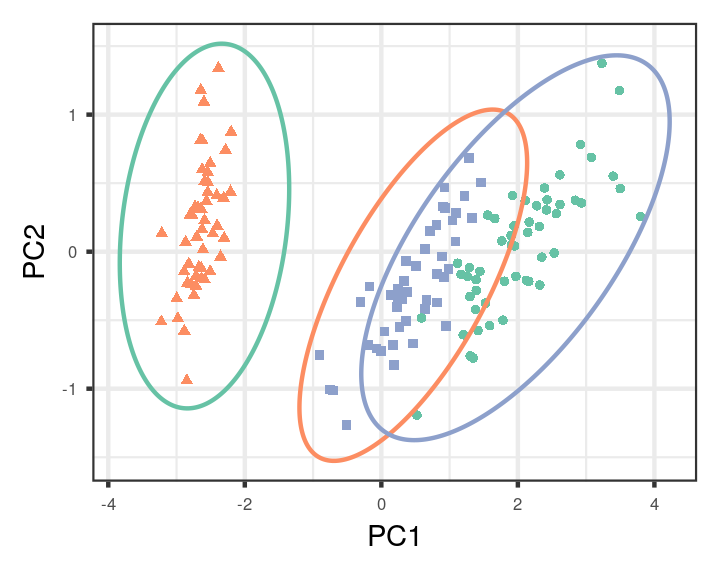
\includegraphics[width=0.588\linewidth,height=0.470\linewidth]{figure/iris_fit-1} 

}

\caption[The iris data in principal component space and 
                      GMM fit at $\alpha = 6$]{The iris data in principal component space and 
                      GMM fit at $\alpha = 6$. 
                      Colors denote inferred memberships and
                      ellipses are estimated covariances. }\label{fig:iris_fit}
\end{figure}


\end{knitrout}

We wish to evaluate the sensitivity of the expected number of clusters to the 
stick-breaking distribution. 
Define the expected number of \textit{in-sample} clusters as
\begin{align*}
\gclusters(\eta) &= \expect{\q(\z\vert\eta)}{\sum_{k=1}^\kmax \ind{ \sum_{n=1}^{N}
\z_{\n\k} > 0}} \\ 
&= \sum_{k=1}^\kmax \left(1 -  \prod_{n=1}^N
\left(1 - \expect{\q(\z_{nk}\vert\eta)}{\z_{nk}}\right)\right).
\end{align*}
The expectation and product can be interchanged because $q$ is mean-field. 

The in-sample quantity $\gclusters$ is an estimate for 
the number of species present in the observed iris dataset. 
Alternatively, we can define a {\itshape posterior predictive} quantity, 
which is an estimate of the number of species one would expect to see 
should a new iris dataset of size $N$ be collected.
Define the posterior predictive number of clusters as 
\begin{align}\eqlabel{post_pred_nclusters}
\gclusterspred(\eta) = \expect{\q(\nu\vert\eta)}{\sum_{k=1}^\kmax\left(1 -
(1 - \pi_k)^N\right)},
\end{align}
where recall that $\pi_k$ are the mixture weights computed from the stick-lengths, $\pi_\k = \nuk \prod_{\k' < \k} (1 - \nu_{\k'})$. 

Unlike the in-sample quantity, the expectation for the predictive quantity is not a simple closed-form function of the variational parameters.  
Instead, we approximate~\eqref{post_pred_nclusters} using Monte Carlo draws from the variational distribution. 
Specifically, we use the ``reparameterization trick" to sample from the variational distribution:
we use an appropriately chosen, $\eta$-dependent transformation 
$f(\cdot, \eta)$ that satisfies 
\begin{align*}
  u \iid\normdist{0, I} \implies 
  f(u, \eta) \stackrel{d}{=} \nu \sim \q(\cdot | \eta).
\end{align*}
To form a Monte Carlo estimate of \eqref{post_pred_nclusters}, 
we sample $u_1, ..., u_m\stackrel{iid}{\sim}\normdist{0, I}$ 
and then average the expression inside the expectation evaluated at points 
$f(u_1, \eta), ..., f(u_m, \eta)$.
We use the reparameterization trick so that conditional on $u_1, ..., u_m$,
our Monte Carlo estimate of $\gclusterspred$ is a determinstic function of 
the variational parameters $\eta$. 
In our experiments below, all displayed values of $\gclusterspred(\eta)$ are
Monte-Carlo approximations, 
conditional on the same $m = 10,000$ draws $u_1, ..., u_m$, fixed a priori. 

We evaluate the sensitivity of the posterior quantities 
$\gclusters$ and $\gclusterspred$ to the prior parameter $\alpha$ in the
$\betadist{\nuk \vert 1, \alpha}$ stick distribution. 
\figref{beta_priors} displays probability density functions of the stick distribution over a range of $\alpha$. 

We fit the initial model at $\alpha = 6$. 
Subsequent refits at $\alpha\not=6$ used the variational parameters at 
$\alpha = 6$ as an initialization. 
As $\alpha$ increases, both the expected in-sample and the expected predictive number of clusters increases (\figref{iris_alpha_sens}). 
The in-sample quantity is relatively insensitive to changes in the $\alpha$ parameter. 
As $\alpha$ varies from $\alpha = 1, ..., 16$, $\gclusters$ varies 
only from 3.0 to 3.4 (recall that the true number of iris species is three). 
On the other hand, the posterior preditive quantity is sensitive 
to changes in $\alpha$.
Over the same range of $\alpha$, $\gclusterspred$ varies from 
3.6 to 8.1. 

We computed the linear approximation at $\alpha = 6$.  
The linear approximation is able to reproduce changes to both 
the in-sample and predictive quantities found by refitting the model at each
$\alpha = 1, ..., 16$ (\figref{iris_alpha_sens}).  
Furthermore, the linear approximation is an order of magnitude faster than refitting. 
Forming the linear approximation, which requires a Hessian inversion (\eqref{vb_eta_sens}), required 0.02 seconds. 
After forming the linear approximation at $\alpha = 6$,
computing $\etalin(\alpha)$ for all $\alpha = 1, ... 16$ took another 
0.02 seconds.
On the other hand, to refit $\etaopt(\alpha)$ for the same range of
$\alpha$'s took a total of 10 seconds, 
with a median refit time of 0.7 seconds. 




\begin{knitrout}
\definecolor{shadecolor}{rgb}{0.969, 0.969, 0.969}\color{fgcolor}\begin{figure}[!h]

{\centering 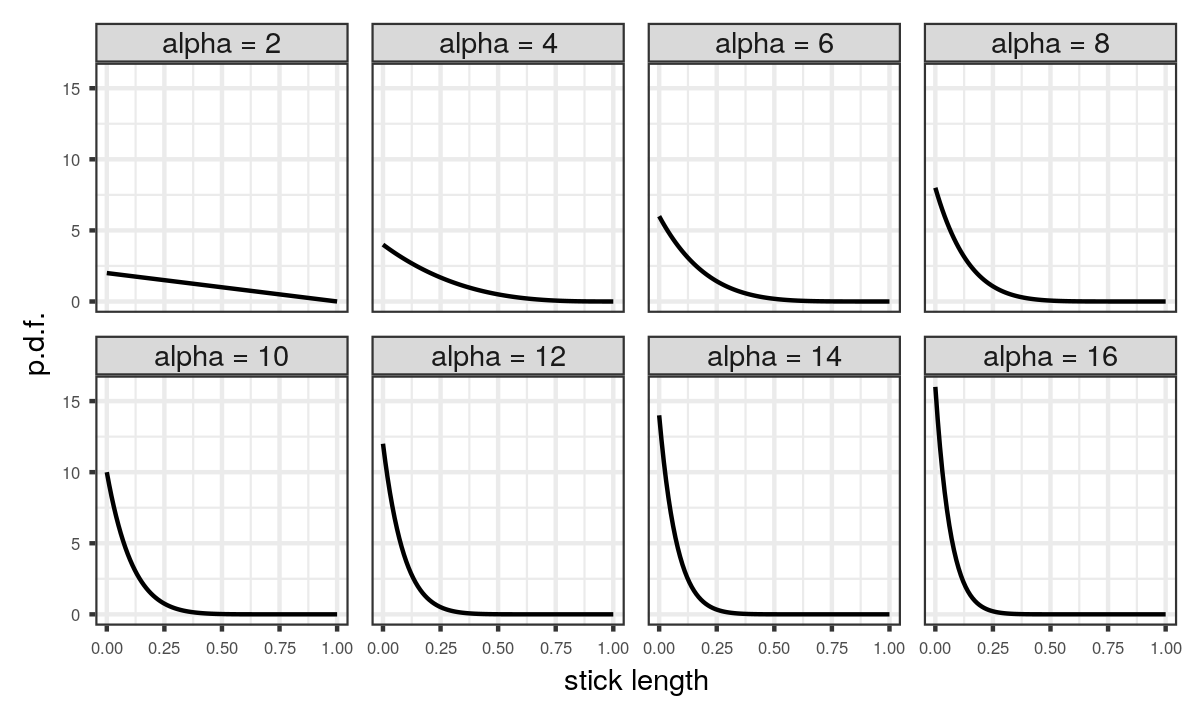
\includegraphics[width=0.980\linewidth,height=0.588\linewidth]{figure/beta_priors-1} 

}

\caption[Probability density functions of $\text{Beta}(1, \alpha)$ distributions, for various $\alpha$]{Probability density functions of $\text{Beta}(1, \alpha)$ distributions, for various $\alpha$. }\label{fig:beta_priors}
\end{figure}


\end{knitrout}




\begin{knitrout}
\definecolor{shadecolor}{rgb}{0.969, 0.969, 0.969}\color{fgcolor}\begin{figure}[!h]

{\centering 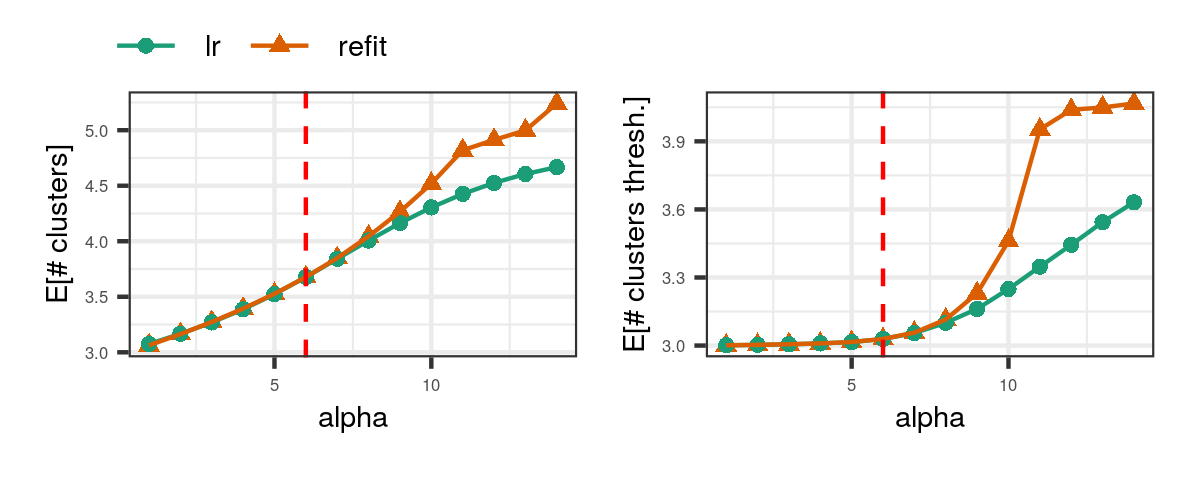
\includegraphics[width=0.980\linewidth,height=0.392\linewidth]{figure/iris_alpha_sens-1} 

}

\caption[The expected number of clusters as $\alpha$ varies in the 
the BNP-GMM fit of the iris data]{The expected number of clusters as $\alpha$ varies in the 
the BNP-GMM fit of the iris data. 
On the left is the sensitivity of the in-sample quantity.  
On the right is the the predictive quantity. 
We compute the linear approximation at $\alpha=6$ and
extrapolate the expected number of clusters using the
linear approximation (green).
We compare against the expected number of clusters obtained by refitting the model at each $\alpha$ (orange). }\label{fig:iris_alpha_sens}
\end{figure}


\end{knitrout}


% 
% - we demonstrate the utility of the influence function 
% - figure ref top three rows shows three different functional perturbations. 
% - can't really tell from densities how these will affect posterior statistic
% - but they do in fact have very different effects (in sign and size). 
% - but their effects make sense when looking at the influence function
% 
% -last row is worst-case

We next consider functional perturbations, 
and we demonstrate the ability of the influence function to 
provide guidance on the anticipated effect of perturbations 
on the posterior quantity. 
Each row of \figref{iris_fsens} presents a different 
multiplicative perturbation $\phi$ to the initial $\betadist{1, 6}$ stick distribution. 
The left column of \figref{iris_fsens} displays the perturbation $\phi$ overlayed with the prior-weighted influence function for $\gclusters$.
The perturbations are of the form 
$\log \phi(x) = e^{2(x - \mu)^2}$, with each perturbation having a 
different value of $\mu$. 
The middle column displays the initial density,
$p_0(\nu_k) = \betadist{\nu_k\vert 1, 6}$, along with the perturbed density,
$p_1(\nu_k) = \betadist{\nu_k\vert 1, 6}\phi(\nu_k)$.

Each perturbation $\phi$ produces distinct changes in the expected number of in-sample clusters $\gclusters$ (\figref{iris_fsens} right column). 
The changes in $\gclusters$ after each perturbation are 
different in both sign and magnitude. 
By examining the perturbed densities alone, it is difficult to anticipate 
the effect of the perturbation on $\gclusters$. 
However, the sign and magnitude of the change in $\gclusters$ is well-explained by the influence function. 
When $\log\phi$ is centered at a location where the influence function is negative, the effect on $\gclusters$ is negative (top row); 
conversely, when $\log\phi$ is centered at a location where the influence function is positive, the effect on $\gclusters$ is positive (bottom row); finally, when $\log\phi$ is centered at a location where the influence is both negative and positive, the effects cancel, and the change in the posterior statistic is roughly zero (middle row). 
In each case, the linear approximation is able to capture the changes in the posterior statistic. 
In applications below, we use influence function to guide our choice of functional perturbaton and to explain why some perturbations result in greater sensitivity than others. 

Finally, we consider the 
worst-case perturbation with unit $L_\infty$ norm.
Recall that the worst-case perturbation with unit $L_\infty$ norm is a 
step-function taking on values $\pm1$ corresponding 
to the sign of the influence function (\figref{iris_worstcase} left).  
The middle column of \figref{iris_worstcase} shows the prior density perturbed by the worst-case perturbation; 
the right column shows the effect on $\gclusters$. 
We see that this worst-case perturbation has a much larger effect on
$\gclusters$ compared to the other unit $L_\infty$ norm perturbations in
\figref{iris_fsens}. 
However, even with the worst-case perturbation, 
the change in $\gclusters$ is still small;
we thus conclude that in the iris dataset $\gclusters$ appears to be a quantity insensitive to the prior. 



\begin{knitrout}
\definecolor{shadecolor}{rgb}{0.969, 0.969, 0.969}\color{fgcolor}\begin{figure}[!h]

{\centering 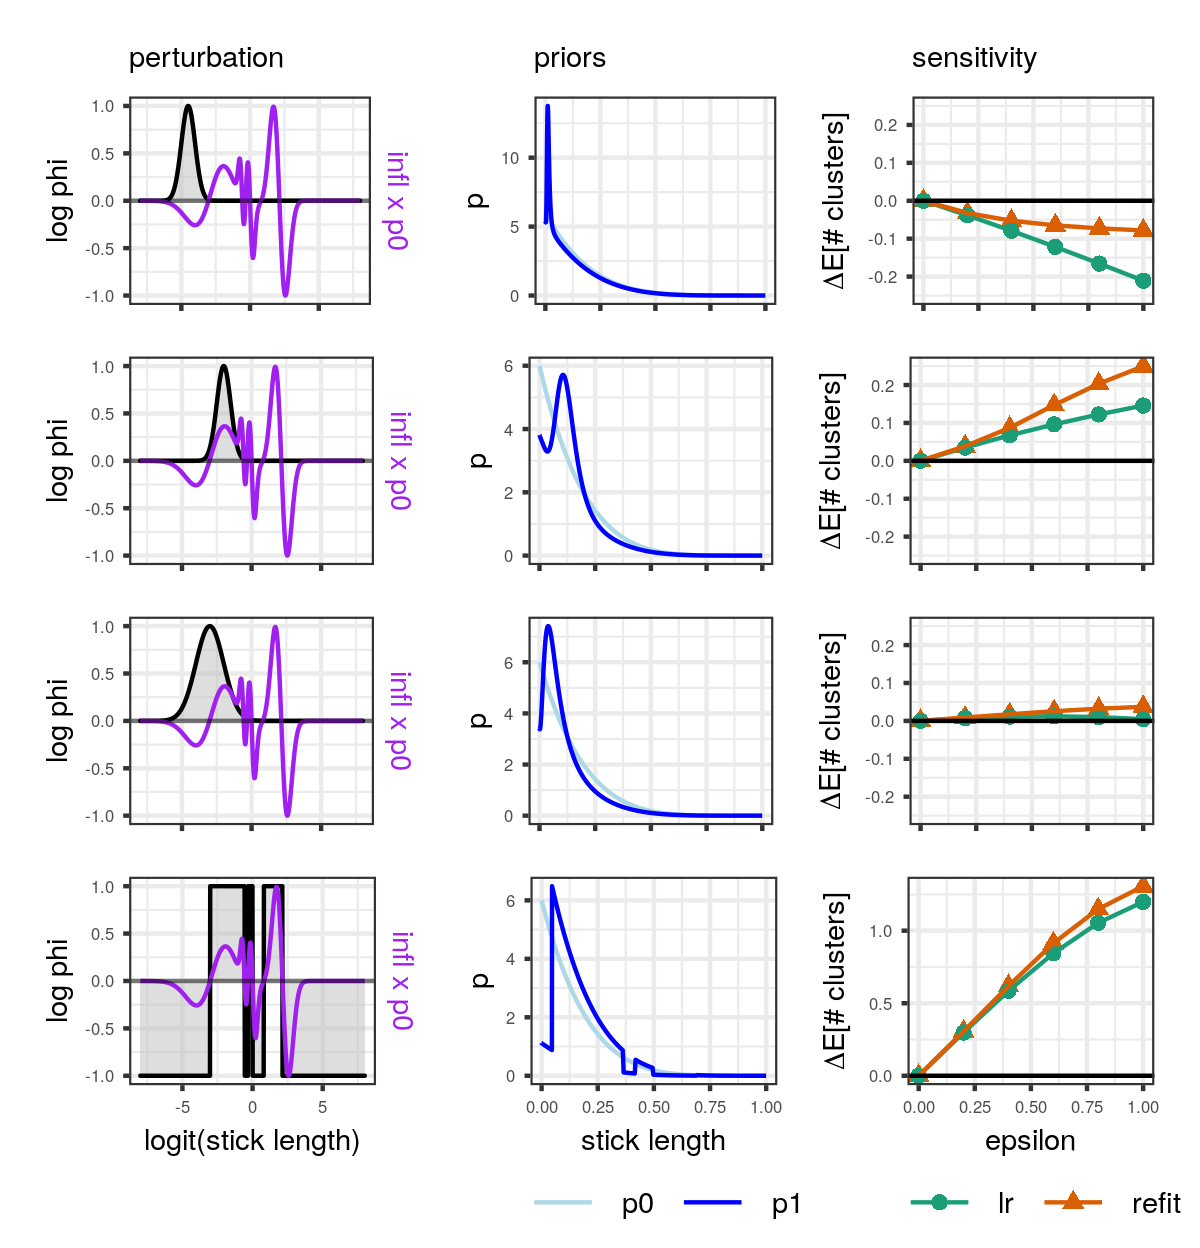
\includegraphics[width=0.980\linewidth,height=0.862\linewidth]{figure/iris_fsens-1} 

}

\caption{Sensitivity of
        the expected number of in-sample clusters in the iris dataset
        to three multiplicative perturbations with 
        unit $L_{\infty}$-norm 
        (Left) The log multiplicative perturbation $\log\phi$ in grey.        
        In purple is the prior-weighted influence function, scaled to also have 
        unit $L_{\infty}$-norm. 
        (Middle) The original prior density $p_0$ and 
        the perturbed prior density $p_1 = p_0\times \phi$. 
        (Right) The effect of the perturbation 
        on the change in expected number of clusters as a function of $\epsilon$. }\label{fig:iris_fsens}
\end{figure}


\end{knitrout}


\begin{knitrout}
\definecolor{shadecolor}{rgb}{0.969, 0.969, 0.969}\color{fgcolor}\begin{figure}[!h]

{\centering 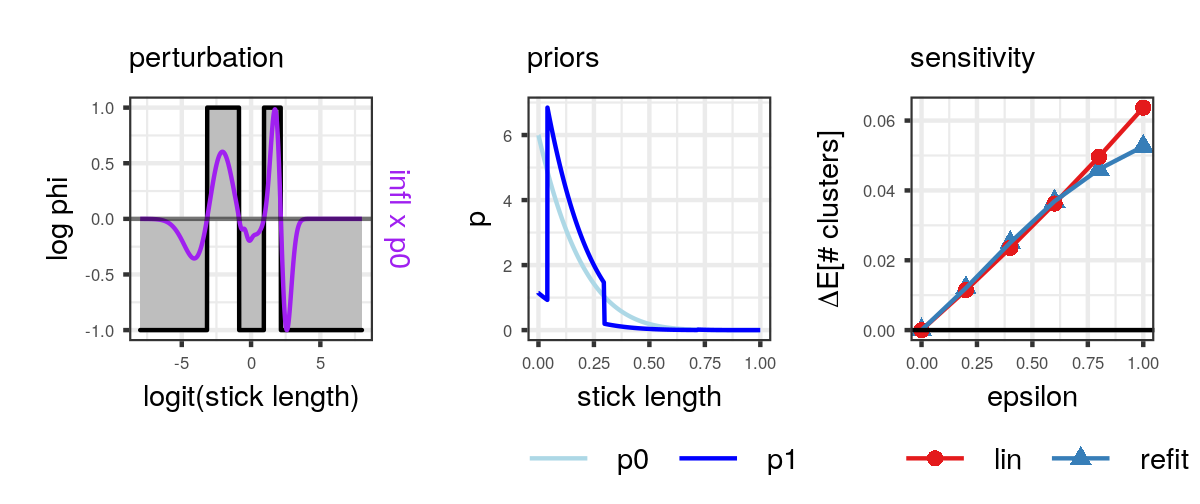
\includegraphics[width=0.980\linewidth,height=0.412\linewidth]{figure/iris_worstcase-1} 

}

\caption[Sensitivity of
        the expected number of in-sample clusters in the iris dataset
        to the worst-case multiplicative perturbations with 
        unit $L_{\infty}$-norm]{Sensitivity of
        the expected number of in-sample clusters in the iris dataset
        to the worst-case multiplicative perturbations with 
        unit $L_{\infty}$-norm.}\label{fig:iris_worstcase}
\end{figure}


\end{knitrout}

% \begin{table}[tb]
% \centering
% \caption{Compute time of results on the iris dataset. }
% \begin{tabular}{|r|r|}
%     \hline 
%     & time (seconds) \\ 
%     \hline 
%     Initial fit & sprintf('%1.2g', init_fit_time) \\
%     \hline 
%     Hessian solve for $\alpha$ sensitivity & 
%         sprintf('%1.2g', alpha_hess_time)\\
%     Linear approx. $\eta^{lin}(\alpha)$ for $\alpha = 1, ... , 16$ & 
%         sprintf('%1.2g', total_alpha_lr_time)\\
%     Refits $\eta(\alpha)$ for $\alpha = 1, ... , 16$ & 
%         sprintf('%1.2g', total_alpha_refit_time)\\
%     \hline 
%     The influence function & sprintf('%1.2g', infl_time)\\ 
%     Hessian solve for worst-case $\phi$ & 
%         sprintf('%1.2g', wc_hessian_time)\\
%     Linear approx. $\eta^{lin}(\epsilon)|_{\epsilon = 1}$
%     for worst-case $\phi$ & 
%         sprintf('%1.2g', wc_lr_time)\\
%     Refit $\eta(\epsilon)|_{\epsilon = 1}$ for worst-case $\phi$ & 
%         sprintf('%1.2g', wc_refit_time)\\ 
%     \hline 
% \end{tabular}
% \end{table}



\section{Results}

\subsection{Regression mixture modeling}
%%%%%%%%%%%%%%%%%%%%%%%%%%%%%%%%%%%%%%
%%%%%%%%%%%%%%%%%%%%%%%%%%%%%%%%%%%%%%
% Do not edit the TeX file your work
% will be overwritten.  Edit the RnW
% file instead.
%%%%%%%%%%%%%%%%%%%%%%%%%%%%%%%%%%%%%%
%%%%%%%%%%%%%%%%%%%%%%%%%%%%%%%%%%%%%%



We consider the problem of clustering time-course gene expression data. 
While thousands of genes might be simultaneously 
measured in a given genomics experiment, 
many genes may exhibit similar expression patterns.  
Clustering gene expressions
is one way to reduce the dimensionality of a complex data set 
and to facilitate scientific interpretations of intricate biological processes. 
Often, such dimensionality reduction is used for exploratory analysis and
is a first step before further downstream investigation.  
It is important, therefore, to acertain the stability of the 
discovered clusters. 
 
We study a publicly available data set of mice gene expression
\citep{shoemaker:2015:ultrasensitive}.
Mice were infected with different influenza viruses, and expression levels of a set of genes were assessed at 14 time points after infection.
Our analysis focuses on mice treated with the ``A/California/04/2009'' strain. 
We normalize the data as described in
\citet{shoemaker:2015:ultrasensitive} and then apply the differential
analysis tool EDGE \citep{Storey:2005:significance} to rank the genes from most to least significantly differentially expressed. 
We fit a BNP model and run our analysis below on the top $\ngenes = 1000$ genes.

\subsubsection*{The model}

Each gene consists of $\ntimepoints = 42$ measurements of expression: three measurements (called biological replicates) at 14 unique timepoints.
The timepoints are unevenly spaced, with more frequent observations at the beginning. 
Following \citet{Luan:2003:clustering} we apply cubic B-splines to smooth the time course expression data. 
Specifically, we model the first 11 timepoints using
cubic B-splines with 7 degrees of freedom.
For the last three timepoints, $\timeindx = 72, 120, 168$ hours,
we use indicator functions. 
That is, if $\tilde \regmatrix$ is the design 
matrix where each column is a
B-spline basis vector evaluated at the $\ntimepoints$ measurement times, 
we append to $\tilde \regmatrix$ three additional columns: 
in these columns, entries are 1
if $\timeindx = 72, 120,$ or 168, repectively, and 0 otherwise. 
Call the full design matrix $\regmatrix$. 
We use indicators for the last three timepoints for numerical stability; 
without the indicator columns,
the matrix $\tilde \regmatrix^T \tilde \regmatrix$ is nearly singular
because the later timepoints are more spread out. 
See \figref{example_genes} for an example gene and the B-spline basis. 

%

\begin{knitrout}
\definecolor{shadecolor}{rgb}{0.969, 0.969, 0.969}\color{fgcolor}\begin{figure}[!h]

{\centering 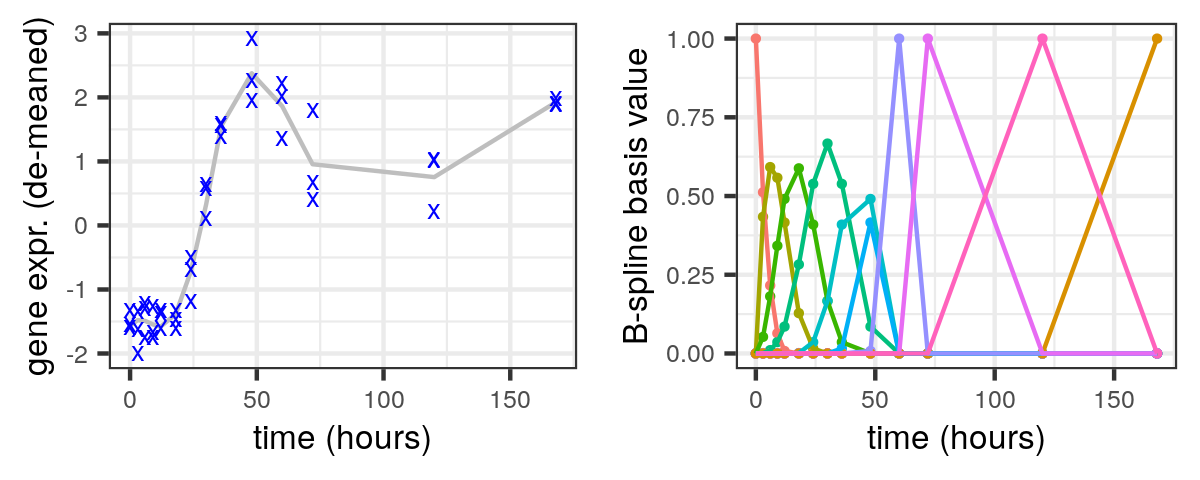
\includegraphics[width=0.980\linewidth,height=0.392\linewidth]{figure/example_genes-1} 

}

\caption[(Left) An example gene and its expression measured at 14 unique timepoints
    with three biological replicates at each timepoint.
     (Right) The cubic B-spline basis with 7 degrees of freedom, 
    along with three indicator functions for the last three timepoints, 
    $\timeindx = 72, 120, 168$]{(Left) An example gene and its expression measured at 14 unique timepoints
    with three biological replicates at each timepoint.
     (Right) The cubic B-spline basis with 7 degrees of freedom, 
    along with three indicator functions for the last three timepoints, 
    $\timeindx = 72, 120, 168$.}\label{fig:example_genes}
\end{figure}


\end{knitrout}
%


Let $\x_\n$ be the vector of observations for gene $\n$,
$(\x_{\n 1}, ..., \x_{\n \ntimepoints})^T$.
Each cluster is characterized by a vector of regression coefficients 
$\beta_k$ and a variance $\tau^{-1}_k$; 
the cluster parameters are $\theta_k = (\beta_k, \tau_k)$. 
The distribution of the data arising from cluster $k$ is 
\begin{align*}
\p(\x_\n | \theta_k, \b_{n}) = 
\normdist{\x_\n | \regmatrix\beta_k + \b_{n},
\tau_k^{-1}I_{\ntimepoints \times \ntimepoints}},
\end{align*}
where $\b_{n}$ is a gene-specific additive offset. 
We include the additive offset because we 
are interested in clustering the pattern of gene expression, 
not the absolute level. 

The joint distribution can be written in the same form as~\eqref{bnp_model}, 
except that the conditional log-likelihood also conditions on $b_n$, 
and we also include an additional prior term:
\begin{align*}
\MoveEqLeft
\logp(\x, \theta, \z, \nu) ={}
\nonumber\\&
    \sum_{n=1}^N \sum_{k=1}^{\kmax}
        \z_{\n\k} \left(
            \logp(\x_n \vert \theta_\k, \b_n) + \logp(\b_n) + \log \pi_\k
        \right) +
    \sum_{k=1}^{\kmax} \left(
        \log \pstick(\nuk) + \logp(\theta_\k)
    \right).
\end{align*}
We use a normal prior for the shifts $\b_n$, 
a multivariate normal prior for the coefficients $\beta_n$,
and a gamma prior for the inverse variance $\tau$. 

Our variational distribution factorizes as~\eqref{vb_mf}
with the addition
of a factor for the additive shift: 
\begin{align*}
\q(\zeta \vert \eta) =
    \left( \prod_{\k=1}^{\kmax - 1} \q(\nuk \vert \eta) \right)
    \left( \prod_{\k=1}^{\kmax} \q(\theta_\k \vert \eta) \right)
    \left( \prod_{\n=1}^{\N} \q(\z_{\n} \vert \eta) 
    \q(\b_{\n} \vert \z_{\n}, \eta)\right).
\end{align*}
Note that the variational distribution for $\b_\n$ conditions on $\z$.
We set $\q(\b_{\n} \vert \z_{\n} = k, \eta)$ to be Gaussian
with variational parameters dependent on $\k$. 
For simplicity in this application,
we let $\q(\theta_\k \vert \eta) = \delta (\theta_k \vert \eta)$, 
where $\delta(\cdot \vert \eta)$ denotes a point mass at a parameterized location. 

By parameterizing 
$\q(\z_{\n}, \b_{\n} \vert \eta) = \q(\z_{\n} \vert \eta)  \q(\b_{\n} \vert \z_{\n}, \eta)$ 
the optimal variational parameters for $\q(\z_{\n}, \b_{\n} \vert \eta)$ 
have a closed form given $\q(\nu, \theta \vert \eta)$. See \secref{put_in_appendix}. Therefore, our model fits the global/local framework as discussed in ... 
\todo{need to work on a section that talks about this}

We fitted the initial approximate posterior at $\alpha_0 = 6$. 
\figref{gene_centroids} shows the inferred smoothers 
$\regmatrix\mathbb{E}_\q[\beta_k]$ for selected clusters. 
\figref{gene_initial_coclustering} displays the inferred co-clustering matrix
$\coclusteringmatr(\eta)$, whose $(i,j)$-th entry is the
posterior probability that gene $i$ belongs to the same cluster
as gene $j$, given by 
\begin{align*}
\coclusteringmatr_{ij}(\eta) 
&= \expect{\q(\z\vert\eta)}{\ind{\z_{i} = \z_{j}}} \\
&= \sum_{k=1}^{\kmax}\left(\expect{\q(\z_i\vert\eta)}{\z_{ik}}
\expect{\q(\z_j\vert\eta)}{\z_{jk}}\right).
\end{align*}

Below, we evaluate the sensitivity of the inferred co-clustering matrix to 
both parametric and functional perturbations to the stick distribution. 


\begin{knitrout}
\definecolor{shadecolor}{rgb}{0.969, 0.969, 0.969}\color{fgcolor}\begin{figure}[!h]

{\centering 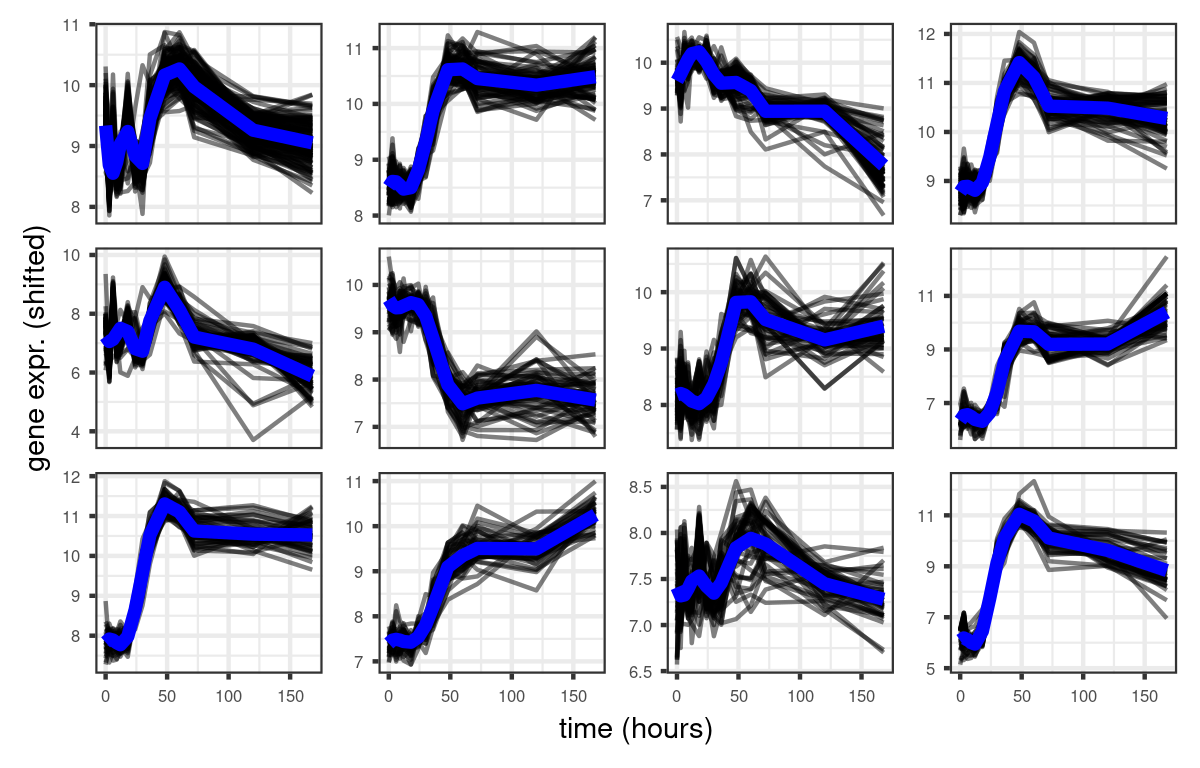
\includegraphics[width=0.980\linewidth,height=0.627\linewidth]{figure/gene_centroids-1} 

}

\caption[Inferred clusters in the mice gene expression dataset]{Inferred clusters in the mice gene expression dataset. 
    Shown are the twelve most occupied clusters. 
    In blue, the inferred cluster centroid. 
    In grey, gene expressions averaged over replicates and
    shifted by their inferred intercepts. }\label{fig:gene_centroids}
\end{figure}


\end{knitrout}



\begin{knitrout}
\definecolor{shadecolor}{rgb}{0.969, 0.969, 0.969}\color{fgcolor}\begin{figure}[!h]

{\centering 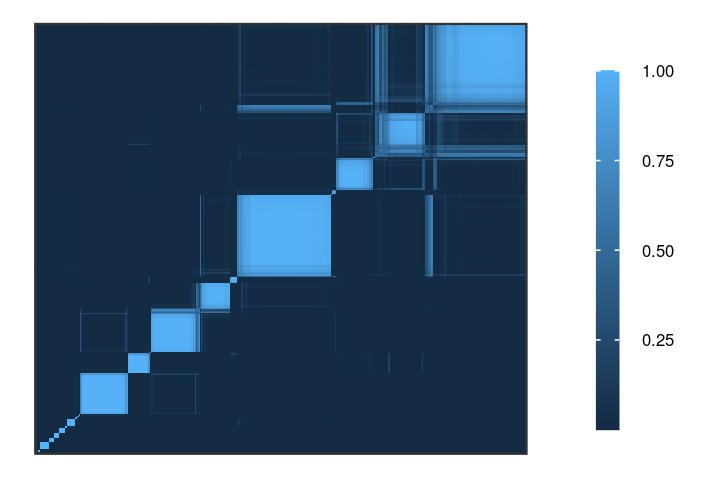
\includegraphics[width=0.588\linewidth,height=0.400\linewidth]{figure/gene_initial_coclustering-1} 

}

\caption[The inferred co-clustering matrix of gene expressions at $\alpha_0 = 6.$ ]{The inferred co-clustering matrix of gene expressions at $\alpha_0 = 6.$ }\label{fig:gene_initial_coclustering}
\end{figure}


\end{knitrout}


\subsubsection*{Sensitivity analysis}

We first evaluate the sensitivity of the co-clustering matrix $\coclusteringmatr$ 
to the choice of $\alpha$ in the
$\betadist{\nuk \vert 1, \alpha}$ stick distribution. 
Let $\coclusteringmatr_0 := \coclusteringmatr(\etaopt(\alpha_0))$ be the co-clustering matrix inferred at $\alpha_0$, 
and let $\Delta\coclusteringmatr(\eta) := 
\coclusteringmatr(\eta) - \coclusteringmatr_0$ be 
the difference in co-clustering matices after a change in the variational parameters $\eta$. 
We formed the linear approximation at $\alpha_0$ and computed
the change in co-clustering under the linearly approximated 
variational parameters, 
$\Delta\coclusteringmatr(\etalin(\alpha))$, at $\alpha = 1$ and $\alpha = 11$. 
For either $\alpha$, the change in the co-clustering matrix 
is miniscule (\figref{gene_alpha_coclustering}):
the largest entry of either matrix $\Delta\coclusteringmatr(\etalin(1))$ 
or $\Delta\coclusteringmatr(\etalin(11))$ is of order $10^{-2}$. 
Refitting the approximate posterior at $\alpha = 1$ and $\alpha = 11$ 
and computing $\Delta\coclusteringmatr(\etaopt(\alpha))$
confirms the insensitivity predicted by the linear approximation. 
Beyond capturing insensitivity, the linear approximation was also able to
approximate the sign and size of the changes in the individual entries of the coclustering matrix (these changes abeit small).  


\begin{knitrout}
\definecolor{shadecolor}{rgb}{0.969, 0.969, 0.969}\color{fgcolor}\begin{figure}[!h]

{\centering 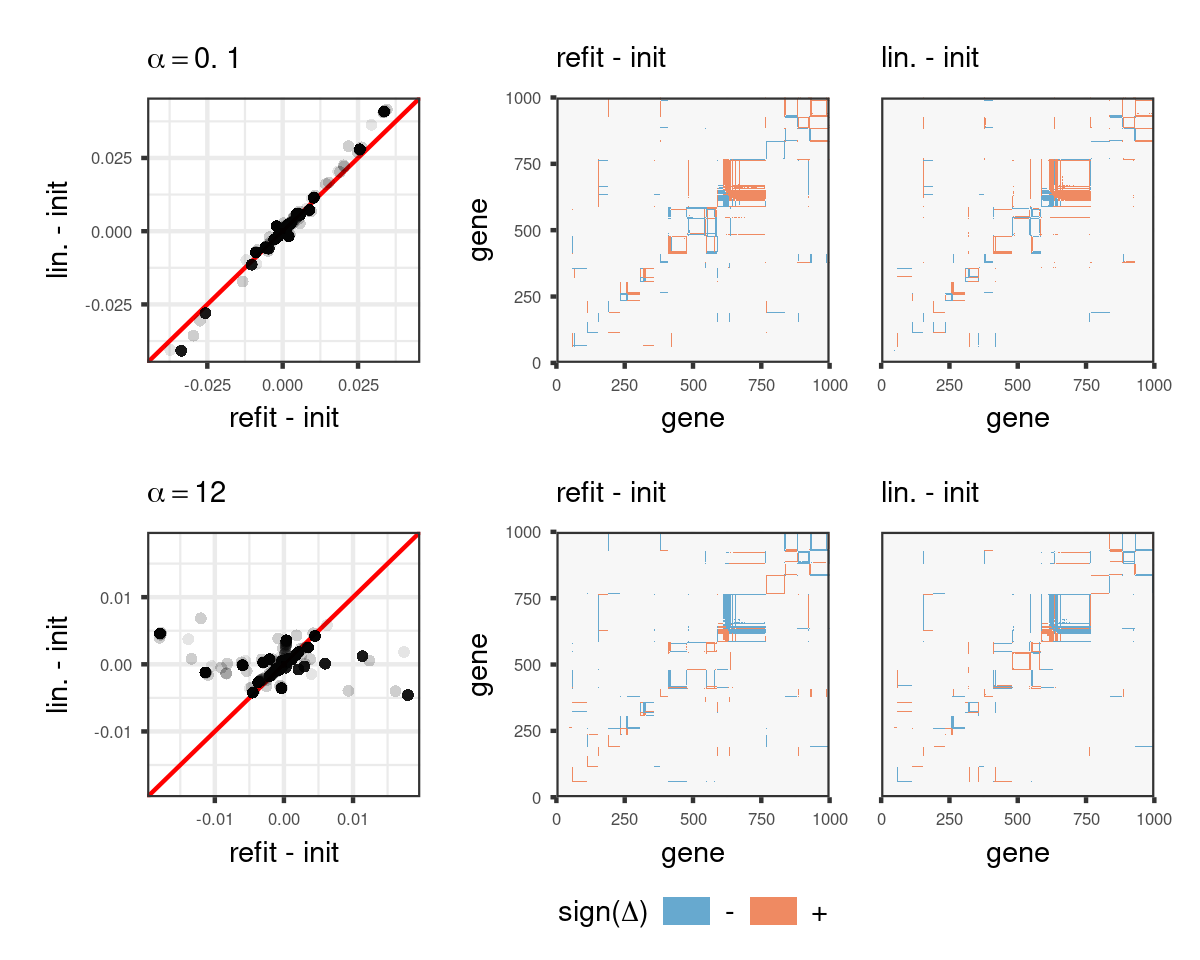
\includegraphics[width=0.980\linewidth,height=0.784\linewidth]{figure/gene_alpha_coclustering-1} 

}

\caption[Differences in the 
     co-clustering matrix at $\alpha = 1$ (top row)
     and $\alpha = 11$ (bottom row),
     relative to the co-clustering matrix at $\alpha_0 = 6$.
     We compare differences obtained with the linearly approximated 
     variational parameters against changes observed after 
     refiting]{Differences in the 
     co-clustering matrix at $\alpha = 1$ (top row)
     and $\alpha = 11$ (bottom row),
     relative to the co-clustering matrix at $\alpha_0 = 6$.
     We compare differences obtained with the linearly approximated 
     variational parameters against changes observed after 
     refiting. 
     (Left) a scatter plot of differences under the linear approximation 
     against differences after refitting, where
     each point represents an entry of the co-coclustering matrix.
     (Middle) the difference in co-clustering matrix observed after refitting. 
     (Right) the difference observed under the linearly approximated variational
     parameters. 
     For visualization, values in the heatmaps
     are clipped at $\pm 10^{-3}$. }\label{fig:gene_alpha_coclustering}
\end{figure}


\end{knitrout}


Insensitivity to $\alpha$ does not necessarily rule out insensitivity to other prior perturbations, however. 
As demonstrated in \secref{results_iris},
the influence function can provide guidance on which functional perturbations may result in greater sensitivity for a chosen posterior quantity. 
However, the co-clustering matrix as a posterior quantity is 
$\ngenes^2$-dimensional and 
thus does not lend itself to an easily interpretable influence function. 
We therefore summarize the co-clustering matrix into a scalar quantity: 
we use the sum of the eigenvalues of the symmetrically normalized graph Laplacian. 
This quantity has close connection with 
the number of distinct components in a graph CITE. 
Let this posterior quantity be denoted $\laplacianevsum$, given by 
\begin{align*}
  \laplacianevsum(\eta) = 
  \text{Tr}\left(
  I - D(\eta)^{-1/2} \coclusteringmatr(\eta) D(\eta)^{-1/2}
  \right),
\end{align*}
where $D(\eta)^{-1/2}$ is the diagonal matrix with entries $d_i = \sum_{j=1}^{\ngenes}[\coclusteringmatr(\eta)]_{ij}$. 
(And recall that the trace of a matrix is equivalent to the sum of its eigenvalues).

Because $\laplacianevsum(\eta)$ is a scalar quantity, we can plot its influence function. 
We choose a functional perturbation $\log\phi_{\textrm{ev}}$ that has a large, positive inner-product with the influence function.
In this case, we construct $\log\phi_{\textrm{ev}}$
using two Gaussian bumps aligned with
the two largest modes of the prior-weighted influence function
(\figref{gene_fpert_coclustering} top left). 
We anticipate $\log\phi_{\textrm{ev}}$
to have a large effect on $\laplacianevsum$. 
With $\laplacianevsum$ a proxy for our actual posterior quantity of interest, 
the full co-clustering matrix, we then expect that the co-clustering matrix 
will also experience large changes. 





Our intuition is confirmed in \figref{gene_fpert_coclustering}. 
After perturbing by $\log\phi_{\textrm{ev}}$, 
the largest changes in the co-clustering matrix are of now of order $10^{-1}$, 
compared with changes on the order of $10^{-2}$ after the $\alpha$ perturbations. 
The linear approximation again able to capture the qualitative changes in the co-clustering matrix after refitting at the perturbed prior. 


\begin{knitrout}
\definecolor{shadecolor}{rgb}{0.969, 0.969, 0.969}\color{fgcolor}\begin{figure}[!h]

{\centering 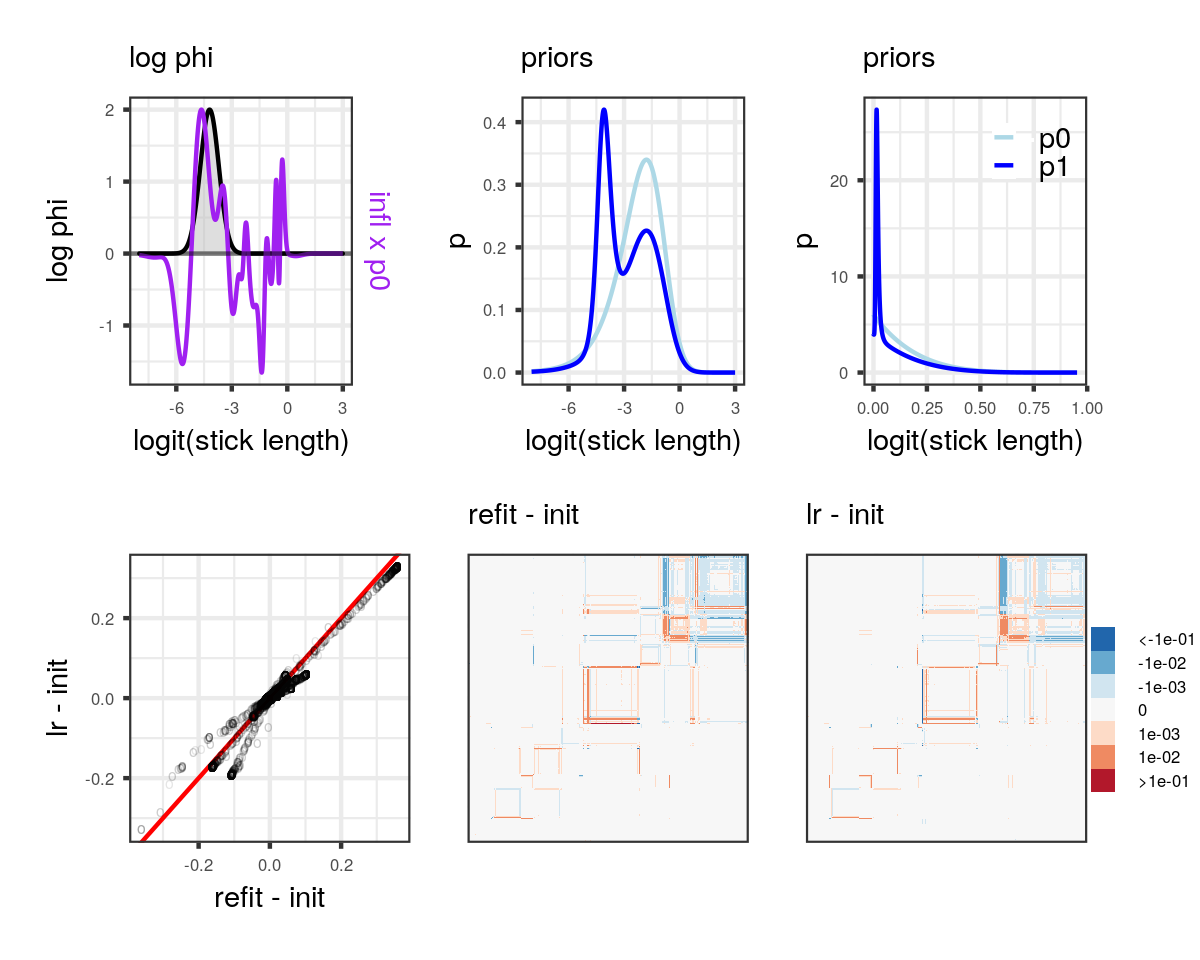
\includegraphics[width=0.980\linewidth,height=0.784\linewidth]{figure/gene_fpert_coclustering-1} 

}

\caption[Effect on the co-clustering matrix after a multiplicative functional
     perturbation.
     The perturbation $\phi$ (top left, in grey) 
     is a difference of two Gaussian bumps 
     scaled to have $L_\infty$ norm equal to two.
     $\phi$ is chosen such that the Gaussian bumps roughly align with the 
     two largest modes of the influence function (top left, purple]{Effect on the co-clustering matrix after a multiplicative functional
     perturbation.
     The perturbation $\phi$ (top left, in grey) 
     is a difference of two Gaussian bumps 
     scaled to have $L_\infty$ norm equal to two.
     $\phi$ is chosen such that the Gaussian bumps roughly align with the 
     two largest modes of the influence function (top left, purple; 
     the influence function is scaled to also have $L_\infty$ norm equal to two).
     The effect of this perturbation on the prior density in the top right. 
     The bottom row shows the effect of this perturbation on 
    the coclustering matrix.
    For visualization, the differences in the heatmap 
     are clipped at $\pm 10^{-1}$.}\label{fig:gene_fpert_coclustering}
\end{figure}


\end{knitrout}

The influence function is able to explain why the co-clustering matrix is 
insensitive to $\alpha$.
The functional perturbation
that corresponds to a change in $\alpha$ is
\begin{align*}
\log \phi_\alpha(\nu_\k) :=
\log\betadist{\nu_\k\vert 1, \alpha} -
\log\betadist{\nu_\k\vert 1, \alpha_0}.
\end{align*}
The function $\log\phi_\alpha(\nu_\k)$ is large when the influence function is small and vice-versa (\figref{alpha_pert_logphi}),
resulting in a small inner-product between the influence function
and $\log\phi_\alpha$. 
Thus, the linear approximation will predict small changes, and 
the refitted results confirms the linear approximation predictions. 


\begin{knitrout}
\definecolor{shadecolor}{rgb}{0.969, 0.969, 0.969}\color{fgcolor}\begin{figure}[!h]

{\centering 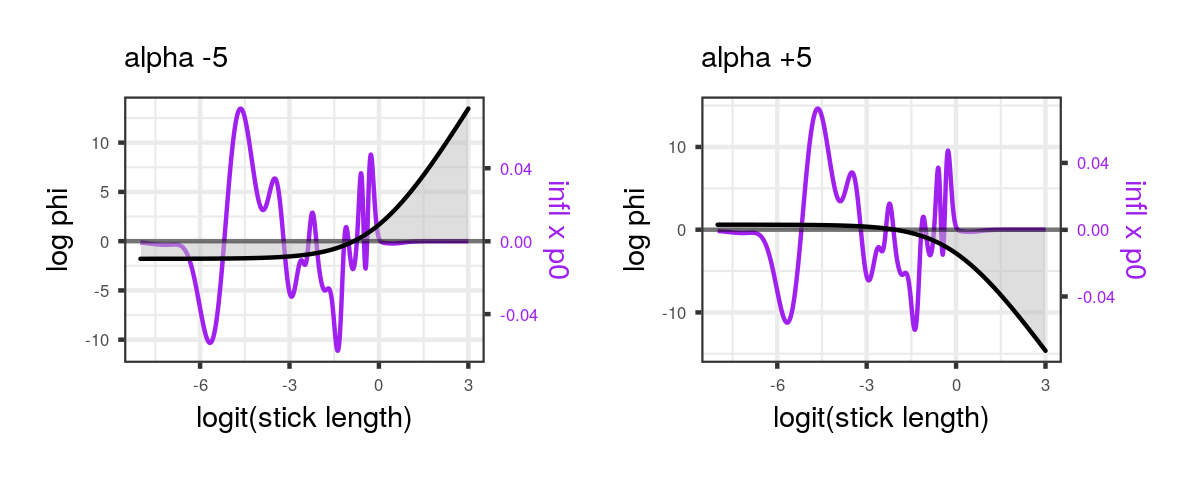
\includegraphics[width=0.882\linewidth,height=0.423\linewidth]{figure/alpha_pert_logphi-1} 

}

\caption[The multiplicative perturbations $\phi_\alpha(\cdot)$ that 
    corresponds to decreasing (left) or increasing (right) 
    the $\alpha$ parameter by five]{The multiplicative perturbations $\phi_\alpha(\cdot)$ that 
    corresponds to decreasing (left) or increasing (right) 
    the $\alpha$ parameter by five. }\label{fig:alpha_pert_logphi}
\end{figure}


\end{knitrout}

However, even with the selected functional perturbation,
the size of the differences in the co-clustering matrix remains modest. 
It is unlikely that any conclusions derived from the co-clustering matrix would have changed after the functional perturbation. 
The co-clustering matrix appears insensitive to perturbations in the stick-breaking distribution. 

Finally, we note that the computational cost of the linear approximation is again favorable compared with refitting (\tabref{mice_timing}). 
Forming the linear approximation, which requires a Hessian inversion, 
took 3-4 seconds; subsequent evaluations of $\etalin$ take milliseconds. 
Conversely, refitting the model after a prior perturbation can take up to 20 seconds. 

\begin{table}[tb]
\centering
\caption{Compute time of results on the mice data set. }
\tablabel{mice_timing}
\begin{tabular}{|r|r|}
    \hline 
    & time (seconds) \\ 
    \hline 
    Initial fit & 30 \\
    \hline 
    Hessian solve for $\alpha$ sensitivity & 
        3.9\\
    Linear approx. $\eta^{lin}(\alpha)$ for $\alpha = 1$ & 
        0.0013\\
    Linear approx. $\eta^{lin}(\alpha)$ for $\alpha = 11$ & 
        0.0012\\
    Refit $\eta(\alpha)$ for $\alpha = 1$ & 
        14\\
    Refit $\eta(\alpha)$ for $\alpha = 11$ & 
        13\\
    \hline
    The influence function & 4.3\\ 
    Hessian solve for $\phi$ perturbation &
        3.3\\
    Linear approx. $\eta^{lin}(\epsilon)$ at $\epsilon = 1$ &
        0.00099\\
    Refit $\eta(\epsilon)$ at $\epsilon = 1$ &
        22\\
    \hline
\end{tabular}
\end{table}


\subsection{Genetic admixture modeling with STRUCTURE}
%%%%%%%%%%%%%%%%%%%%%%%%%%%%%%%%%%%%%%
%%%%%%%%%%%%%%%%%%%%%%%%%%%%%%%%%%%%%%
% Do not edit the TeX file your work
% will be overwritten.  Edit the RnW
% file instead.
%%%%%%%%%%%%%%%%%%%%%%%%%%%%%%%%%%%%%%
%%%%%%%%%%%%%%%%%%%%%%%%%%%%%%%%%%%%%%



Our final data analysis example is an application of a Bayesian topic model to
population genetics. We consider a publicly available dataset from
\citet{galbusera:2000:thrush} that contains genotypes from 155 samples of an
endangered bird species, the Taita thrush. Individuals were collected from four
regions in southeast Kenya (Chawia, Mbololo, Ngangao, Yale), and each individual
was genotyped at seven micro-satellite loci. The four regions were once part of
a cohesive cloud forest that has since been fragmented by human development. For
this endangered bird species, understanding the degree to which populations have
grown genetically distinct is important for conservation efforts: well-separated
populations with little genetic diversity are particularly at risk of
extinction.  The goal of the analysis is to identify the presence of latent
populations, from which one can infer the population of origin for specific
loci, and estimate the degree to which populations are admixed in each
individual.


\subsubsection*{The model}

The data consists of consists of $\nindiv$ individuals genotyped at $\nloci$
loci. Let $\x_{\n\l\i}\in\{1, \ldots, J_\l\}$ be the observed genotype for
individual $\n$ at locus $\l$ and chromosome $\i$. $J_\l$ is the number of
possible genotypes at locus $\l$. For example, if the measurements are all
single nucleotides (A, T, C or G) then $J_\l = 4$ for all $\l$.

A latent population is characterized by the collection $\beta_k =
(\latentpop_{\k1}, \ldots, \latentpop_{\k\nloci})$ where
$\latentpop_{\k\l}\in\Delta^{J_\l - 1}$ are the latent frequencies for the $J_l$
possible genotypes at locus $\l$. Let $\z_{\n\l\i}$ be the assignment of
observation $\x_{\n\l\i}$ to a latent population. Notice that for a given
individual $\n$, different loci, or even different chromosomes at a given locus,
may have different population assignments. The distribution of
$\x_{\n\l\i}\in\{1, \ldots, J_\l\}$ arising from population $\k$ is
%
\begin{align*}
\p(\x_{\n\l\i} \vert \latentpop_{\k}) =
\categoricaldist{\x_{\n\l\i}\vert \latentpop_{\k\l}}.
\end{align*}

Unlike the previous models, we now have a stick-breaking process for each
individual. Draw sticks
%
\begin{align*}
\nu_{\n\k} \iid \pstick(\nu_{\n\k}) \quad \forall \n = 1, \ldots, \nindiv; \k = 1, 2, \ldots \infty.
\end{align*}
%
The prior assignment probability vector $\latentadmix_{\n} =
(\latentadmix_{\n1}, \latentadmix_{\n2}, \ldots)$, now unique to each
individual, is formed by the same stick-breaking construction as before,
%
\begin{align*}
\latentadmix_{\n\k} = \nu_{\n\k} \prod_{\k' < \k} (1 - \nu_{\n\k'}).
\end{align*}
%
The population assignment $\z_{\n\l\i}$ is drawn from the usual multinomial
distribution
%
\begin{align*}
p(\z_{\n\l\i} | \latentadmix_\n) = \prod_{k=1}^{\infty} \latentadmix_{\n\k}^{\z_{\n\l\i\k}}.
\end{align*}
%
In this genetics application, we call $\latentadmix_{\n}$ the \textit{admixture}
of individual $\n$.

This model is identical to fastSTRUCTURE, a model proposed in
\citet{pritchard:2000:structure, raj:2014:faststructure}, except that we replace
the Dirichlet prior in fastSTRUCTURE with an infinite stick-breaking process.
The result is a model similar to a hierarchical Dirichlet process for topic
modeling \citep{teh:2006:hdp}, but without the top-level Dirichlet process. In
addition, genotypes at genetic markers take the place of words in a document; in
lieu of inferring ``topics," we infer latent populations.

The variational approximation is mean-field as before, and all distributions are
conditionally conjugate except for the stick-breaking proportions, which remain
logit-normal. See \appref{app_structure} for further details.



\begin{knitrout}
\definecolor{shadecolor}{rgb}{0.969, 0.969, 0.969}\color{fgcolor}\begin{figure}[!h]

{\centering 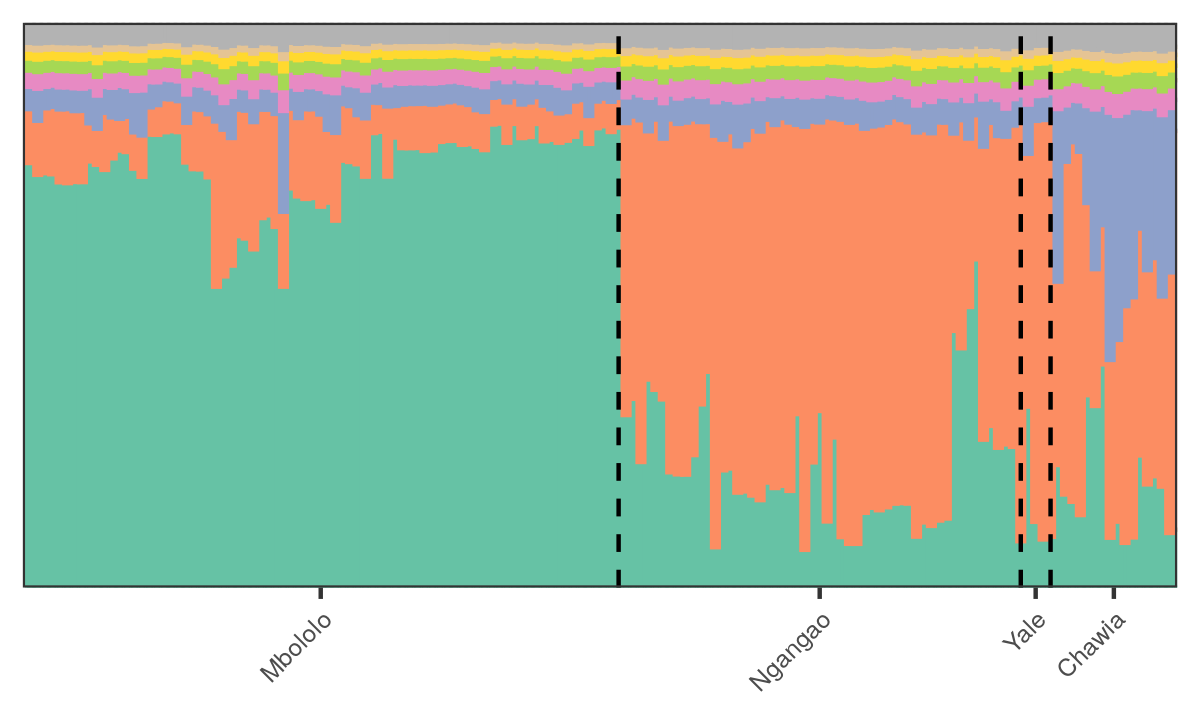
\includegraphics[width=0.980\linewidth,height=0.588\linewidth]{figure/stru_init_fit-1} 

}

\caption[The inferred individual admixtures at $\alpha_0 = 3$.
    Each vertical strip is an individual and each color
    a latent population.
    Lengths of colored segments represent the inferred admixture proportions.
    Individuals are ordered by the geographic region from which they were sampled
    (Mbololo, Ngangao, Yale, and Chawia).
    In the text, we refer to the green, orange, and purple latent populations
    as population 1, 2, and 3, respectively]{The inferred individual admixtures at $\alpha_0 = 3$.
    Each vertical strip is an individual and each color
    a latent population.
    Lengths of colored segments represent the inferred admixture proportions.
    Individuals are ordered by the geographic region from which they were sampled
    (Mbololo, Ngangao, Yale, and Chawia).
    In the text, we refer to the green, orange, and purple latent populations
    as population 1, 2, and 3, respectively. }\label{fig:stru_init_fit}
\end{figure}


\end{knitrout}

\subsubsection*{Quantity of interest}

The posterior quantities of interest in this application
are the individual admixtures $\pi_\n$.
\figref{stru_init_fit} plots the inferred admixtures $\pi_\n$ for all
individuals $\n$ under a $\gem$ prior with parameter $\alpha_0 = 3$.
The choice of $\alpha_0 = 3$ corresponds to roughly four distinct populations {\em a priori}, motivated by the fact that the individuals come from four geographic regions.
We will examine the robustness of the inferred admixtures to the prior below.

In the posterior at $\alpha_0$, there
appear to be three dominant latent populations, which we arbitrarily label as
populations 1, 2, and 3 (\figref{stru_init_fit}).
The inferred admixture proportions generally correspond with the geographic regions from which each individuals are sampled.

Notably, outlying admixtures among individuals from the same geographic region provide clues into the historical migration patterns of this species.
For example,
while individuals collected from the Mbololo region are inferred to be admixed
primarily with population 1, several individuals from this region have
abnormally large admixture proportions of population 2. Conversely, while
individuals collected from the Ngangao region are admixed primarily with
population 2, a few of these individuals have abnormally large admixture
proportions of population 1. This suggests that some migration has occurred
between the Mbololo and Ngangao regions.

We evaluate the sensitivity of this conclusion to possible prior perturbations.
Consider the posterior statistic
%
\begin{align*}
\gadmix(\eta; \mathcal{N}, k) =
 \expect{\q(\pi\vert\eta)}{\frac{1}{|\mathcal{N}|}\sum_{n\in\mathcal{N}}
\pi_{\n\k}},
\end{align*}
%
the average admixture proportion of population $\k$ in a set of
individuals $\mathcal{N}$.

Below, we present results on three variations of $\gadmix$, corresponding to
indididuals hightlighted as ``A," ``B", or ``C" in the top row of \figref{stru_func_sens}:
$\mathcal{N} = \{26, ..., 31\}$ and $k = 2$,
corresponding to the six individuals from the Mbololo region with outlying proportions of population 2;
$\mathcal{N} = \{125, ..., 128\}$ and $k = 1$,
corresponding to the four individuals from the Ngangao region with outlying proportions of population 1;
$\mathcal{N} = \{139, ..., 155\}$ and $k = 3$,
corresponding to all individuals from the Chawia region.
The first two posterior quantities relate to the inferred migration between
the Mbololo and Ngangao regions.
In the last case, we are studying the robustness of having a third latent
population present, a population which primarily appears in Chawia individuals.

\subsubsection*{Functional sensitivity}

In \figref{stru_func_sens}, we construct the worst-case negative perturbation
for decreasing each of our three variant of $\gadmix$, in order to see
whether the biologically interesting patterns can be made to disappear
with different prior choices.

\todo{Make the text easier to match up with the picture, which doesn't
have the populations (Ngangao, etc) labeled.  Right now it's hard to see
what's going on.}

\todo{I think this whole section could be easier to understand and much more
compact.  Basically just say that A is non-robust, B is robust, and on C
the linear approximation and refit disagree.  Then we investigate A more.}

Under the
linearized variational parameters $\etalinglobal(\t)$, the admixture proportion
of population 2 in the outlying Mbololo individuals is nearly halved.
The same quantity computed after refitting the model confirms the
sensitivity predicted by the linearized variational parameters.

 On the other
hand, the presence of population 1 in the outlying Ngangao individuals appears
to be insensitive even after this worst-case perturbation. The linearized and
the refitted variational parameters again agree on this conclusion. Finally, the
presence of population 3 in the Chawia individuals is anticipated to be
sensitive by the linearized parameters, as this admixture proportion steadily
decreases as $t\rightarrow 1$. However, under the refits, this admixture
proportion does not decrease steadily but rather levels off after $t = 0.5$.



\begin{knitrout}
\definecolor{shadecolor}{rgb}{0.969, 0.969, 0.969}\color{fgcolor}\begin{figure}[!h]

{\centering 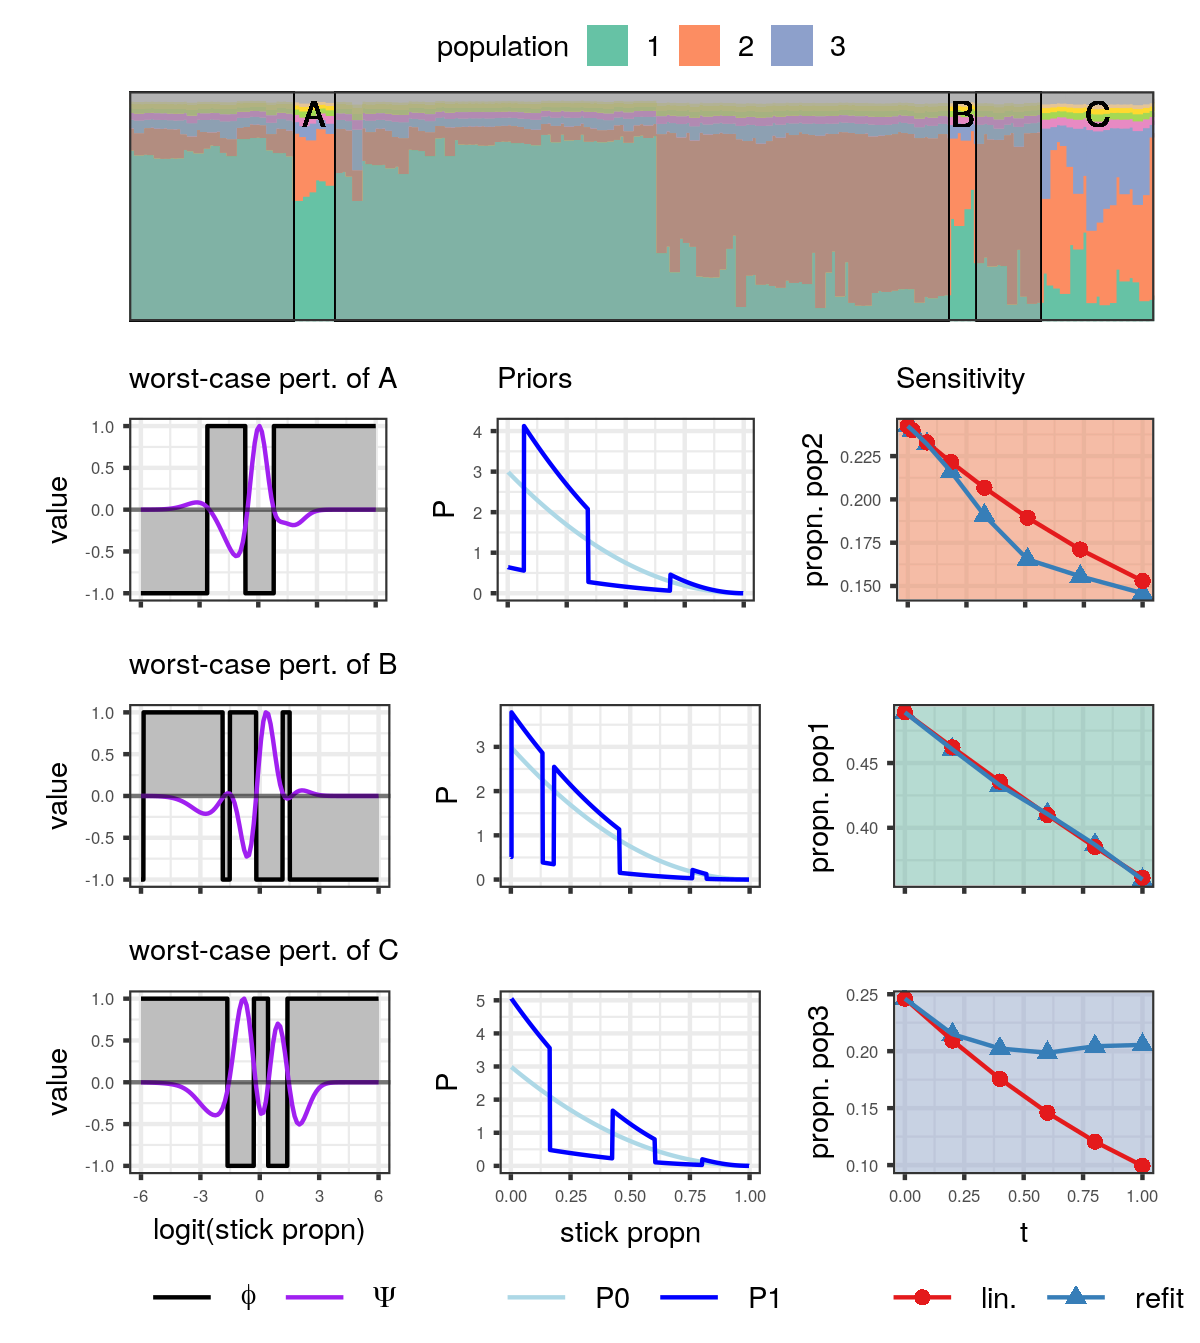
\includegraphics[width=0.980\linewidth,height=1.098\linewidth]{figure/stru_func_sens-1} 

}

\caption[Sensitivity of inferred admixtures for several outlying individuals.
     For individuals A,
     we examine the sensitivity of the admixture proportion of population 2.
     For individuals B,
     we examine the population 1 admixture
     For the individuals C, we examine the population 3 admixture.
     (Left column) The worst-case negative perturbation with
     $\norminf{\phi} = 1$
     in grey,
     plotted against the influence function in purple
     (scaled such that $\norminf{\psi} = 1$).
    (Middle column) The effect of the perturbation on the prior density.
    (Right column) Effects on the inferred admixture]{Sensitivity of inferred admixtures for several outlying individuals.
     For individuals A,
     we examine the sensitivity of the admixture proportion of population 2.
     For individuals B,
     we examine the population 1 admixture
     For the individuals C, we examine the population 3 admixture.
     (Left column) The worst-case negative perturbation with
     $\norminf{\phi} = 1$
     in grey,
     plotted against the influence function in purple
     (scaled such that $\norminf{\psi} = 1$).
    (Middle column) The effect of the perturbation on the prior density.
    (Right column) Effects on the inferred admixture. }\label{fig:stru_func_sens}
\end{figure}


\end{knitrout}


\todo{Say something about the fact that these priors are maybe too
adversarial.}


The conclusions from the linear approximation did not
perfectly agree with the conclusions from refitting variational approximation
in this data set and model.
For example, the admixture proportion of population 3 in individuals ``C" were predicted to be non-robust by our linear approximation but are in actuality are robust after refitting (bottom row \figref{stru_func_sens}).

Moreover, even though the linearized parameters
agreed with the refits in producing the diminished
overall admixture proportion of population 2 in individuals ``A"
(\figref{stru_func_sens} second row),
the approximation does does not perform uniformly well over all individual admixtures.
\figref{stru_func_sens_admix} plots the individual admixtures after the worst-case prior perturbation computed under both our linear approximation and after refitting.
The admixture proportion of population 2 in individual $n = 25$
dramatically increased after refitting with the perturbed prior $\p_1$;
the linearized parameters failed to reproduce this change.
For a more in depth discussion of the limitations of the linear approximation,
see \appref{app_structure_results}.

\todo{need to highlight main takeaway: even though linear approx works less well, still can use influence function to guide where to refit. }


\begin{knitrout}
\definecolor{shadecolor}{rgb}{0.969, 0.969, 0.969}\color{fgcolor}\begin{figure}[!h]

{\centering 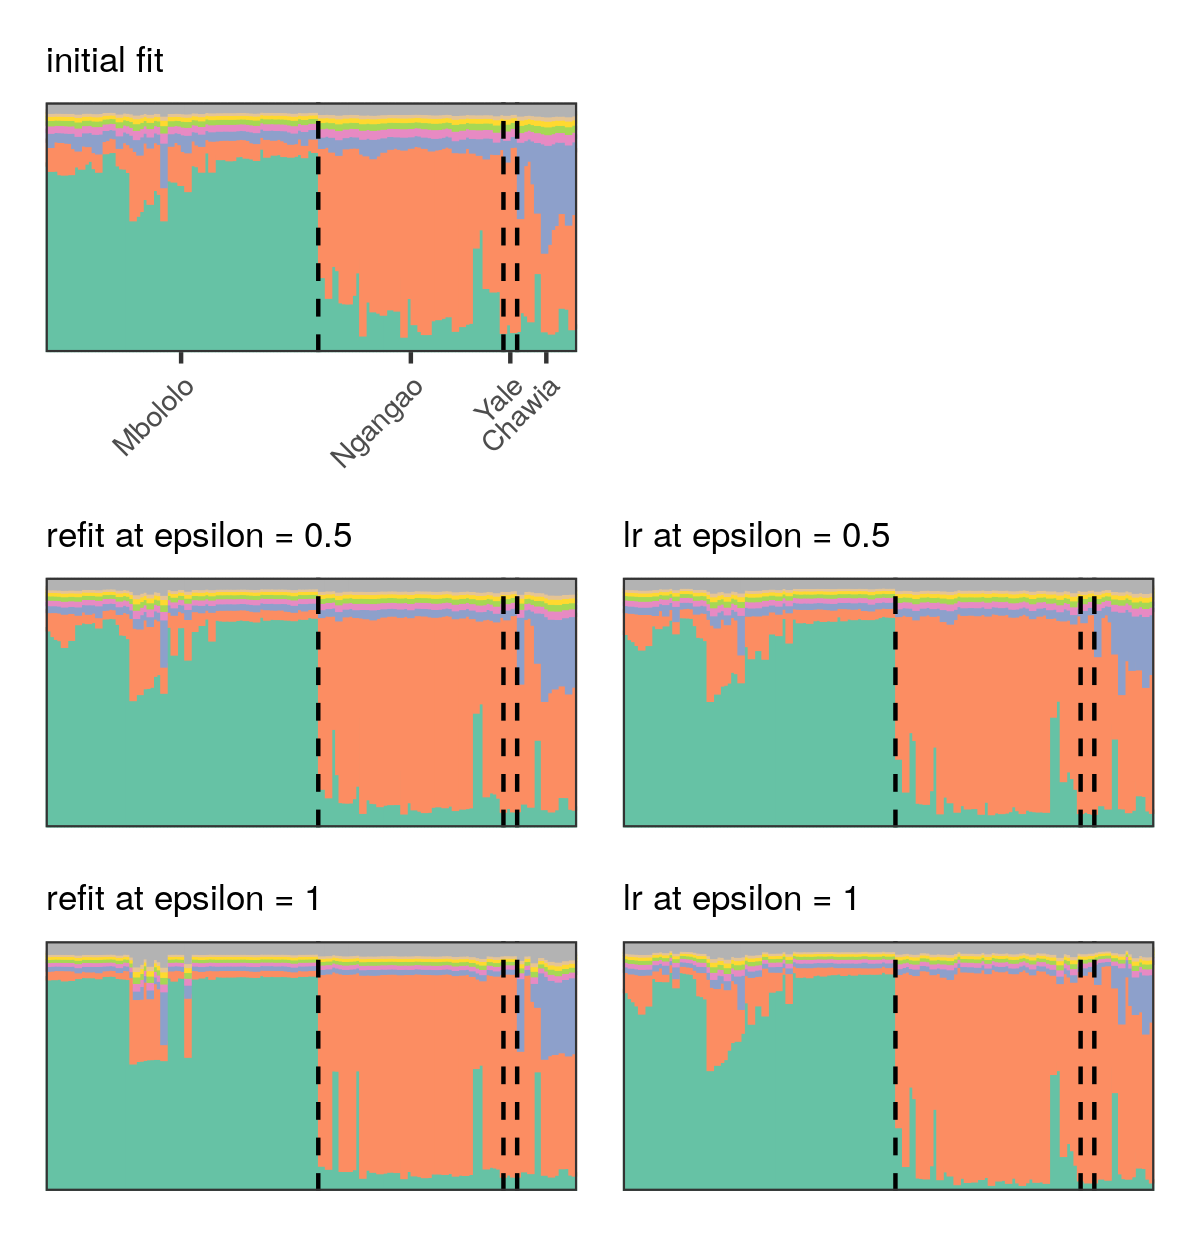
\includegraphics[width=0.980\linewidth,height=0.392\linewidth]{figure/stru_func_sens_admix-1} 

}

\caption{Inferred admixtures after the worst-case perturbation
     to individuals ``A" (see Figure~\ref{fig:stru_func_sens} for perturbation). }\label{fig:stru_func_sens_admix}
\end{figure}


\end{knitrout}


\newcommand{\StructureLimitationsA}{

\begin{knitrout}
\definecolor{shadecolor}{rgb}{0.969, 0.969, 0.969}\color{fgcolor}\begin{figure}[!h]

{\centering 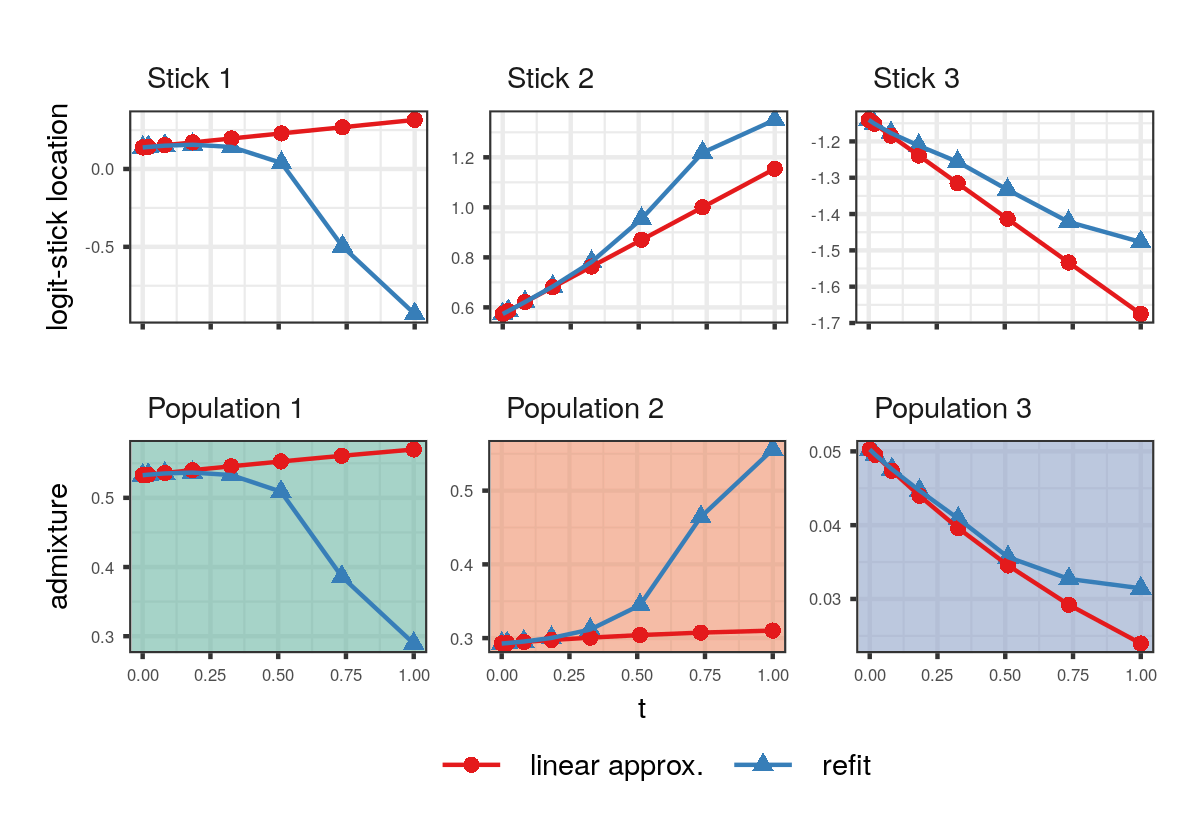
\includegraphics[width=0.980\linewidth,height=0.666\linewidth]{figure/stru_lin_bad_example-1} 

}

\caption[An individual $(\n = 26)$ for which
    the linearly approximated variational parameters
    poorly captured the
    change in admixture observed after refitting
    as $\t \rightarrow 1$.
    (Top row) the change in location parameter of the normally
    distributed logit-sticks, for the first three sticks.
    The response here is a variational parameter, so
    the approximation (red) is necessarily linear with respect to $\t$.
    (Bottom row) the change in the inferred admixtures for
    populations 1, 2, and 3]{An individual $(\n = 26)$ for which
    the linearly approximated variational parameters
    poorly captured the
    change in admixture observed after refitting
    as $\t \rightarrow 1$.
    (Top row) the change in location parameter of the normally
    distributed logit-sticks, for the first three sticks.
    The response here is a variational parameter, so
    the approximation (red) is necessarily linear with respect to $\t$.
    (Bottom row) the change in the inferred admixtures for
    populations 1, 2, and 3. }\label{fig:stru_lin_bad_example}
\end{figure}


\end{knitrout}
}

\newcommand{\StructureLimitationsB}{

\begin{knitrout}
\definecolor{shadecolor}{rgb}{0.969, 0.969, 0.969}\color{fgcolor}\begin{figure}[!h]

{\centering 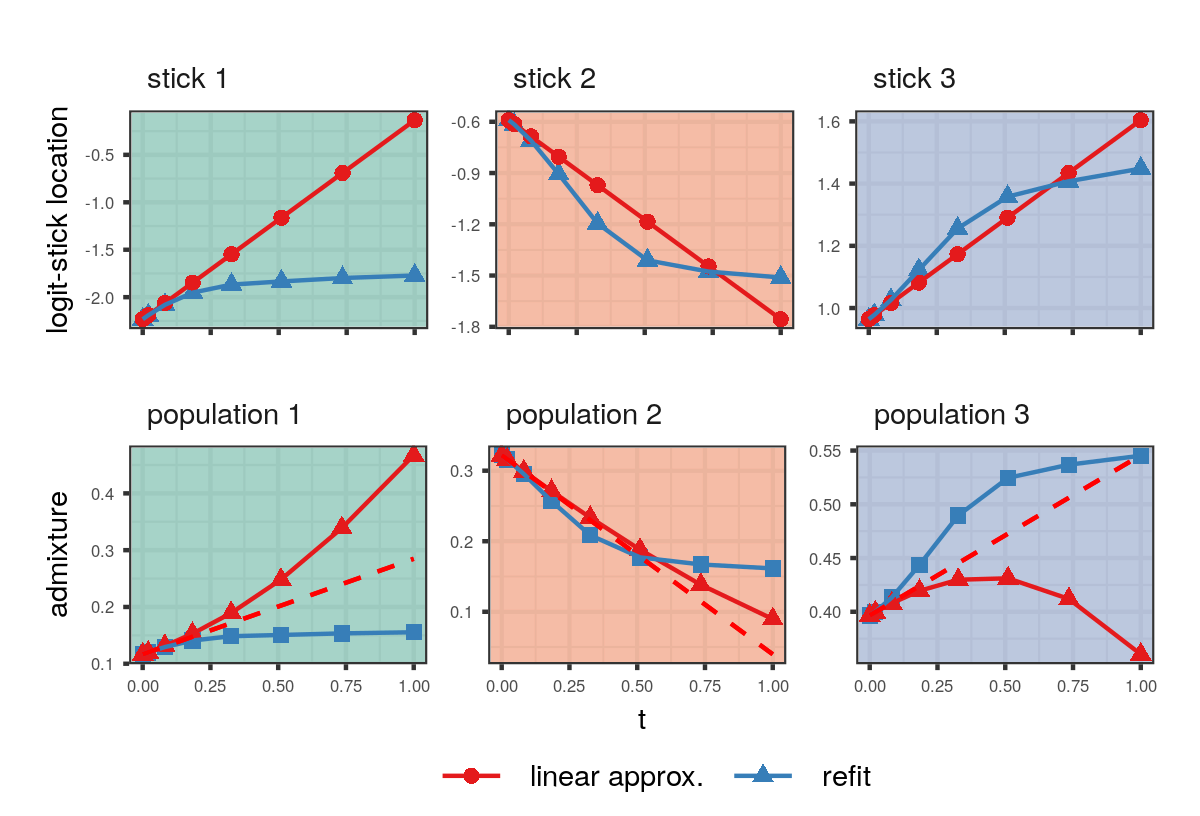
\includegraphics[width=0.980\linewidth,height=0.666\linewidth]{figure/stru_fully_lin_example-1} 

}

\caption[An example where
    linearizing the posterior quantity itself outperforms
    linearizing the variational parameters only.
    Shown are logit-stick location parameters (top row) and
    inferred admixtures (bottom row)
    for individual $n = 74$ and populations $k = 1, 2$ and $3$.
    Dashed red is the approximation $\glin(\t)$ formed by linearizing the
    inferred admixture $\expect{\q}{\pi_{\n\k}}$ with respect to prior
    parameter $t$.
    On the admixture proportion of population 3,
    $\glin(\t)$ outperforms $\g(\etalin(\t))$ (solid red)]{An example where
    linearizing the posterior quantity itself outperforms
    linearizing the variational parameters only.
    Shown are logit-stick location parameters (top row) and
    inferred admixtures (bottom row)
    for individual $n = 74$ and populations $k = 1, 2$ and $3$.
    Dashed red is the approximation $\glin(\t)$ formed by linearizing the
    inferred admixture $\expect{\q}{\pi_{\n\k}}$ with respect to prior
    parameter $t$.
    On the admixture proportion of population 3,
    $\glin(\t)$ outperforms $\g(\etalin(\t))$ (solid red). }\label{fig:stru_fully_lin_example}
\end{figure}


\end{knitrout}
}


\section{Conclusion}
This concludes.


\section{Acknowledgements}
Thanks to everyone.

% Manual newpage inserted to improve layout of sample file - not
% needed in general before appendices/bibliography.

\bibliography{references}
\bibliographystyle{plainnat}


\newpage

\appendix
\section*{Appendix A.}
\label{app:theorem}

Supplemental results

\end{document}
